\documentclass[twoside]{book}

% Packages required by doxygen
\usepackage{fixltx2e}
\usepackage{calc}
\usepackage{doxygen}
\usepackage[export]{adjustbox} % also loads graphicx
\usepackage{graphicx}
\usepackage[utf8]{inputenc}
\usepackage{makeidx}
\usepackage{multicol}
\usepackage{multirow}
\PassOptionsToPackage{warn}{textcomp}
\usepackage{textcomp}
\usepackage[nointegrals]{wasysym}
\usepackage[table]{xcolor}

% NLS support packages
\usepackage[french]{babel}

% Font selection
\usepackage[T1]{fontenc}
\usepackage[scaled=.90]{helvet}
\usepackage{courier}
\usepackage{amssymb}
\usepackage{sectsty}
\renewcommand{\familydefault}{\sfdefault}
\allsectionsfont{%
  \fontseries{bc}\selectfont%
  \color{darkgray}%
}
\renewcommand{\DoxyLabelFont}{%
  \fontseries{bc}\selectfont%
  \color{darkgray}%
}
\newcommand{\+}{\discretionary{\mbox{\scriptsize$\hookleftarrow$}}{}{}}

% Page & text layout
\usepackage{geometry}
\geometry{%
  a4paper,%
  top=2.5cm,%
  bottom=2.5cm,%
  left=2.5cm,%
  right=2.5cm%
}
\tolerance=750
\hfuzz=15pt
\hbadness=750
\setlength{\emergencystretch}{15pt}
\setlength{\parindent}{0cm}
\setlength{\parskip}{0.2cm}
\makeatletter
\renewcommand{\paragraph}{%
  \@startsection{paragraph}{4}{0ex}{-1.0ex}{1.0ex}{%
    \normalfont\normalsize\bfseries\SS@parafont%
  }%
}
\renewcommand{\subparagraph}{%
  \@startsection{subparagraph}{5}{0ex}{-1.0ex}{1.0ex}{%
    \normalfont\normalsize\bfseries\SS@subparafont%
  }%
}
\makeatother

% Headers & footers
\usepackage{fancyhdr}
\pagestyle{fancyplain}
\fancyhead[LE]{\fancyplain{}{\bfseries\thepage}}
\fancyhead[CE]{\fancyplain{}{}}
\fancyhead[RE]{\fancyplain{}{\bfseries\leftmark}}
\fancyhead[LO]{\fancyplain{}{\bfseries\rightmark}}
\fancyhead[CO]{\fancyplain{}{}}
\fancyhead[RO]{\fancyplain{}{\bfseries\thepage}}
\fancyfoot[LE]{\fancyplain{}{}}
\fancyfoot[CE]{\fancyplain{}{}}
\fancyfoot[RE]{\fancyplain{}{\bfseries\scriptsize Généré le Dimanche 13 Décembre 2015 22\+:43\+:07 pour I-\/rover par Doxygen }}
\fancyfoot[LO]{\fancyplain{}{\bfseries\scriptsize Généré le Dimanche 13 Décembre 2015 22\+:43\+:07 pour I-\/rover par Doxygen }}
\fancyfoot[CO]{\fancyplain{}{}}
\fancyfoot[RO]{\fancyplain{}{}}
\renewcommand{\footrulewidth}{0.4pt}
\renewcommand{\chaptermark}[1]{%
  \markboth{#1}{}%
}
\renewcommand{\sectionmark}[1]{%
  \markright{\thesection\ #1}%
}

% Indices & bibliography
\usepackage{natbib}
\usepackage[titles]{tocloft}
\setcounter{tocdepth}{3}
\setcounter{secnumdepth}{5}
\makeindex

% Hyperlinks (required, but should be loaded last)
\usepackage{ifpdf}
\ifpdf
  \usepackage[pdftex,pagebackref=true]{hyperref}
\else
  \usepackage[ps2pdf,pagebackref=true]{hyperref}
\fi
\hypersetup{%
  colorlinks=true,%
  linkcolor=blue,%
  citecolor=blue,%
  unicode%
}

% Custom commands
\newcommand{\clearemptydoublepage}{%
  \newpage{\pagestyle{empty}\cleardoublepage}%
}


%===== C O N T E N T S =====

\begin{document}

% Titlepage & ToC
\hypersetup{pageanchor=false,
             bookmarks=true,
             bookmarksnumbered=true,
             pdfencoding=unicode
            }
\pagenumbering{roman}
\begin{titlepage}
\vspace*{7cm}
\begin{center}%
{\Large I-\/rover \\[1ex]\large 1.\+0 }\\
\vspace*{1cm}
{\large Généré par Doxygen 1.8.9.1}\\
\vspace*{0.5cm}
{\small Dimanche 13 Décembre 2015 22:43:07}\\
\end{center}
\end{titlepage}
\clearemptydoublepage
\tableofcontents
\clearemptydoublepage
\pagenumbering{arabic}
\hypersetup{pageanchor=true}

%--- Begin generated contents ---
\chapter{Index hiérarchique}
\section{Hiérarchie des classes}
Cette liste d\textquotesingle{}héritage est classée approximativement par ordre alphabétique \+:\begin{DoxyCompactList}
\item Application\begin{DoxyCompactList}
\item \contentsline{section}{Map\+Display}{\pageref{classMapDisplay}}{}
\item \contentsline{section}{Map\+Display\+Test\+Pathfinding}{\pageref{classMapDisplayTestPathfinding}}{}
\end{DoxyCompactList}
\item \contentsline{section}{Clef}{\pageref{classClef}}{}
\item \contentsline{section}{Coffre}{\pageref{classCoffre}}{}
\item \contentsline{section}{Map}{\pageref{classMap}}{}
\item \contentsline{section}{node}{\pageref{classnode}}{}
\item \contentsline{section}{Personnage}{\pageref{classPersonnage}}{}
\begin{DoxyCompactList}
\item \contentsline{section}{Ennemi}{\pageref{classEnnemi}}{}
\item \contentsline{section}{Robot}{\pageref{classRobot}}{}
\end{DoxyCompactList}
\item Test\+Case\begin{DoxyCompactList}
\item \contentsline{section}{Test\+Robot}{\pageref{classTestRobot}}{}
\end{DoxyCompactList}
\item \contentsline{section}{Tileset}{\pageref{classTileset}}{}
\end{DoxyCompactList}

\chapter{Index des classes}
\section{Liste des classes}
Liste des classes, structures, unions et interfaces avec une brève description \+:\begin{DoxyCompactList}
\item\contentsline{section}{\hyperlink{classArme}{Arme} }{\pageref{classArme}}{}
\item\contentsline{section}{\hyperlink{classArmure}{Armure} }{\pageref{classArmure}}{}
\item\contentsline{section}{\hyperlink{classBazooka}{Bazooka} }{\pageref{classBazooka}}{}
\item\contentsline{section}{\hyperlink{classClef}{Clef} }{\pageref{classClef}}{}
\item\contentsline{section}{\hyperlink{classCoffre}{Coffre} }{\pageref{classCoffre}}{}
\item\contentsline{section}{\hyperlink{classEnnemi}{Ennemi} }{\pageref{classEnnemi}}{}
\item\contentsline{section}{\hyperlink{classMap}{Map} }{\pageref{classMap}}{}
\item\contentsline{section}{\hyperlink{classMapDisplay}{Map\+Display} }{\pageref{classMapDisplay}}{}
\item\contentsline{section}{\hyperlink{classMapDisplayTestPathfinding}{Map\+Display\+Test\+Pathfinding} }{\pageref{classMapDisplayTestPathfinding}}{}
\item\contentsline{section}{\hyperlink{classMine}{Mine} }{\pageref{classMine}}{}
\item\contentsline{section}{\hyperlink{classnode}{node} }{\pageref{classnode}}{}
\item\contentsline{section}{\hyperlink{classPersonnage}{Personnage} }{\pageref{classPersonnage}}{}
\item\contentsline{section}{\hyperlink{classRobot}{Robot} }{\pageref{classRobot}}{}
\item\contentsline{section}{\hyperlink{classScanner}{Scanner} }{\pageref{classScanner}}{}
\item\contentsline{section}{\hyperlink{classTestRobot}{Test\+Robot} \\*Classe \hyperlink{classTestRobot}{Test\+Robot} }{\pageref{classTestRobot}}{}
\item\contentsline{section}{\hyperlink{classTileset}{Tileset} }{\pageref{classTileset}}{}
\end{DoxyCompactList}

\chapter{Documentation des classes}
\input{classArme}
\input{classArmure}
\input{classBazooka}
\hypertarget{classClef}{}\section{Référence de la classe Clef}
\label{classClef}\index{Clef@{Clef}}
\subsection*{Fonctions membres publiques}
\begin{DoxyCompactItemize}
\item 
\hyperlink{classClef_ad68f9748c13f66f3ec4c361a867b99fa}{Clef} ()
\item 
\hyperlink{classClef_a1c152618762fbf968582413c35ad9b33}{Clef} (int position\+X, int position\+Y, clan\+::\+Image sprite)
\begin{DoxyCompactList}\small\item\em Classe \hyperlink{classClef}{Clef}. \end{DoxyCompactList}\item 
int \hyperlink{classClef_a0f08d48ab630ee0220b6f6699455fc64}{get\+Position\+X} ()
\item 
int \hyperlink{classClef_ae01a85bce2518b739f6e2039df461024}{get\+Position\+Y} ()
\item 
void \hyperlink{classClef_af56e6b306b8628debd7a51db58631e41}{set\+Position\+X} (int x)
\item 
void \hyperlink{classClef_a2a64bb6ec8734bbc41701df247e0dc01}{set\+Position\+Y} (int y)
\item 
void \hyperlink{classClef_a850351cad9bd4421bc35aebe201429d5}{draw} (clan\+::\+Canvas c, int x, int y)
\end{DoxyCompactItemize}


\subsection{Documentation des constructeurs et destructeur}
\hypertarget{classClef_ad68f9748c13f66f3ec4c361a867b99fa}{}\index{Clef@{Clef}!Clef@{Clef}}
\index{Clef@{Clef}!Clef@{Clef}}
\subsubsection[{Clef}]{\setlength{\rightskip}{0pt plus 5cm}Clef\+::\+Clef (
\begin{DoxyParamCaption}
{}
\end{DoxyParamCaption}
)}\label{classClef_ad68f9748c13f66f3ec4c361a867b99fa}
Le constructeur d\textquotesingle{}une clef par défaut. \begin{DoxyReturn}{Renvoie}
\hyperlink{classClef}{Clef} la clef créée. 
\end{DoxyReturn}
\hypertarget{classClef_a1c152618762fbf968582413c35ad9b33}{}\index{Clef@{Clef}!Clef@{Clef}}
\index{Clef@{Clef}!Clef@{Clef}}
\subsubsection[{Clef}]{\setlength{\rightskip}{0pt plus 5cm}Clef\+::\+Clef (
\begin{DoxyParamCaption}
\item[{int}]{x, }
\item[{int}]{y, }
\item[{clan\+::\+Image}]{sprite}
\end{DoxyParamCaption}
)}\label{classClef_a1c152618762fbf968582413c35ad9b33}


Classe \hyperlink{classClef}{Clef}. 

Implémentation de la classe \hyperlink{classClef}{Clef} et de ses méthodes. \begin{DoxyAuthor}{Auteur}
Geoffrey D\+E\+S\+B\+R\+O\+S\+S\+E\+S 
\end{DoxyAuthor}
\begin{DoxyVersion}{Version}
1 
\end{DoxyVersion}
\begin{DoxyDate}{Date}
2015-\/12-\/09
\end{DoxyDate}
Constructeur d\textquotesingle{}une clef. 
\begin{DoxyParams}[1]{Paramètres}
\mbox{\tt in}  & {\em x} & La position en x où la clef sera créée. \\
\hline
\mbox{\tt in}  & {\em y} & La position en y où la clef sera créée. \\
\hline
\mbox{\tt in}  & {\em sprite} & L\textquotesingle{}image de la clef. \\
\hline
\mbox{\tt out}  & {\em position\+X} & La nouvelle position en x de la clef. \\
\hline
\mbox{\tt out}  & {\em position\+Y} & La nouvelle position en y de la clef. \\
\hline
\mbox{\tt out}  & {\em sprite} & Le nouvelle image de la clef. \\
\hline
\end{DoxyParams}
\begin{DoxyReturn}{Renvoie}
\hyperlink{classClef}{Clef} la clef créée. 
\end{DoxyReturn}


\subsection{Documentation des fonctions membres}
\hypertarget{classClef_a850351cad9bd4421bc35aebe201429d5}{}\index{Clef@{Clef}!draw@{draw}}
\index{draw@{draw}!Clef@{Clef}}
\subsubsection[{draw}]{\setlength{\rightskip}{0pt plus 5cm}void Clef\+::draw (
\begin{DoxyParamCaption}
\item[{clan\+::\+Canvas}]{c, }
\item[{int}]{x, }
\item[{int}]{y}
\end{DoxyParamCaption}
)}\label{classClef_a850351cad9bd4421bc35aebe201429d5}
Méthode servant à dessiner une clef sur la map. 
\begin{DoxyParams}[1]{Paramètres}
\mbox{\tt in}  & {\em c} & Le contexte où dessiner. \\
\hline
\mbox{\tt in}  & {\em x} & la position en x de la clef à dessiner. \\
\hline
\mbox{\tt in}  & {\em y} & la position en y de la clef à dessiner. \\
\hline
\mbox{\tt out}  & {\em sprite} & L\textquotesingle{}image de l\textquotesingle{}objet aux coordonnées (x,y). \\
\hline
\end{DoxyParams}
\hypertarget{classClef_a0f08d48ab630ee0220b6f6699455fc64}{}\index{Clef@{Clef}!get\+Position\+X@{get\+Position\+X}}
\index{get\+Position\+X@{get\+Position\+X}!Clef@{Clef}}
\subsubsection[{get\+Position\+X}]{\setlength{\rightskip}{0pt plus 5cm}int Clef\+::get\+Position\+X (
\begin{DoxyParamCaption}
{}
\end{DoxyParamCaption}
)}\label{classClef_a0f08d48ab630ee0220b6f6699455fc64}
Le getter de la position en x de la clef. \begin{DoxyReturn}{Renvoie}
la position courante de la clef en x. 
\end{DoxyReturn}
\hypertarget{classClef_ae01a85bce2518b739f6e2039df461024}{}\index{Clef@{Clef}!get\+Position\+Y@{get\+Position\+Y}}
\index{get\+Position\+Y@{get\+Position\+Y}!Clef@{Clef}}
\subsubsection[{get\+Position\+Y}]{\setlength{\rightskip}{0pt plus 5cm}int Clef\+::get\+Position\+Y (
\begin{DoxyParamCaption}
{}
\end{DoxyParamCaption}
)}\label{classClef_ae01a85bce2518b739f6e2039df461024}
Le getter de la position en y de la clef. \begin{DoxyReturn}{Renvoie}
la position courante de la clef en y. 
\end{DoxyReturn}
\hypertarget{classClef_af56e6b306b8628debd7a51db58631e41}{}\index{Clef@{Clef}!set\+Position\+X@{set\+Position\+X}}
\index{set\+Position\+X@{set\+Position\+X}!Clef@{Clef}}
\subsubsection[{set\+Position\+X}]{\setlength{\rightskip}{0pt plus 5cm}void Clef\+::set\+Position\+X (
\begin{DoxyParamCaption}
\item[{int}]{x}
\end{DoxyParamCaption}
)}\label{classClef_af56e6b306b8628debd7a51db58631e41}
Le setter de la position en x de la clef. Modifie la position de la clef en x. 
\begin{DoxyParams}[1]{Paramètres}
\mbox{\tt in}  & {\em x} & La valeur à affecter à l\textquotesingle{}attribut position\+X de la clef. \\
\hline
\mbox{\tt out}  & {\em position\+X} & la nouvelle position en x de la clef. \\
\hline
\end{DoxyParams}
\hypertarget{classClef_a2a64bb6ec8734bbc41701df247e0dc01}{}\index{Clef@{Clef}!set\+Position\+Y@{set\+Position\+Y}}
\index{set\+Position\+Y@{set\+Position\+Y}!Clef@{Clef}}
\subsubsection[{set\+Position\+Y}]{\setlength{\rightskip}{0pt plus 5cm}void Clef\+::set\+Position\+Y (
\begin{DoxyParamCaption}
\item[{int}]{y}
\end{DoxyParamCaption}
)}\label{classClef_a2a64bb6ec8734bbc41701df247e0dc01}
Le setter de la position en y de la clef. Modifie la position de la clef en y. 
\begin{DoxyParams}[1]{Paramètres}
\mbox{\tt in}  & {\em y} & La valeur à affecter à l\textquotesingle{}attribut position\+Y de la clef. \\
\hline
\mbox{\tt out}  & {\em position\+Y} & la nouvelle position en y de la clef. \\
\hline
\end{DoxyParams}


La documentation de cette classe a été générée à partir des fichiers suivants \+:\begin{DoxyCompactItemize}
\item 
Code\+Main/clef.\+hpp\item 
Code\+Main/clef.\+cpp\end{DoxyCompactItemize}

\hypertarget{classCoffre}{}\section{Référence de la classe Coffre}
\label{classCoffre}\index{Coffre@{Coffre}}
\subsection*{Fonctions membres publiques}
\begin{DoxyCompactItemize}
\item 
\hyperlink{classCoffre_aaec05282cbda83ba82707a492007d7c4}{Coffre} ()
\item 
\hyperlink{classCoffre_a4ab515b02d49013a961784899c65ca9b}{Coffre} (int position\+X, int position\+Y, clan\+::\+Image sprite)
\begin{DoxyCompactList}\small\item\em Classe \hyperlink{classCoffre}{Coffre}. \end{DoxyCompactList}\item 
int \hyperlink{classCoffre_a09119b47a3c3a84401a0f60b0713cf69}{get\+Position\+X} ()
\item 
int \hyperlink{classCoffre_a9623a6bfad74ccb403757bc054cf24dd}{get\+Position\+Y} ()
\item 
bool \hyperlink{classCoffre_a01124ba421e43f7460e3220c227fb7c3}{is\+Ouvert} ()
\item 
void \hyperlink{classCoffre_a514d95ef3c53b50c2a24e97ef4cf49ba}{set\+Position\+X} (int x)
\item 
void \hyperlink{classCoffre_a5e351644ab4ebea39f9ffaf655b97b9b}{set\+Position\+Y} (int y)
\item 
void \hyperlink{classCoffre_ab5d1d8a72878a967e12e96e7226b17f4}{set\+Ouvert} (bool status)
\item 
void \hyperlink{classCoffre_ab54166a456bd84edd5fcb345f6bdd6ef}{draw} (clan\+::\+Canvas c, int x, int y)
\end{DoxyCompactItemize}


\subsection{Documentation des constructeurs et destructeur}
\hypertarget{classCoffre_aaec05282cbda83ba82707a492007d7c4}{}\index{Coffre@{Coffre}!Coffre@{Coffre}}
\index{Coffre@{Coffre}!Coffre@{Coffre}}
\subsubsection[{Coffre}]{\setlength{\rightskip}{0pt plus 5cm}Coffre\+::\+Coffre (
\begin{DoxyParamCaption}
{}
\end{DoxyParamCaption}
)}\label{classCoffre_aaec05282cbda83ba82707a492007d7c4}
Le constructeur d\textquotesingle{}un coffre par défaut. \begin{DoxyReturn}{Renvoie}
\hyperlink{classCoffre}{Coffre} le coffre créé. 
\end{DoxyReturn}
\hypertarget{classCoffre_a4ab515b02d49013a961784899c65ca9b}{}\index{Coffre@{Coffre}!Coffre@{Coffre}}
\index{Coffre@{Coffre}!Coffre@{Coffre}}
\subsubsection[{Coffre}]{\setlength{\rightskip}{0pt plus 5cm}Coffre\+::\+Coffre (
\begin{DoxyParamCaption}
\item[{int}]{x, }
\item[{int}]{y, }
\item[{clan\+::\+Image}]{sprite}
\end{DoxyParamCaption}
)}\label{classCoffre_a4ab515b02d49013a961784899c65ca9b}


Classe \hyperlink{classCoffre}{Coffre}. 

Implémentation de la classe \hyperlink{classCoffre}{Coffre} avec ses méthodes. \begin{DoxyAuthor}{Auteur}
Geoffrey D\+E\+S\+B\+R\+O\+S\+S\+E\+S 
\end{DoxyAuthor}
\begin{DoxyVersion}{Version}
1 
\end{DoxyVersion}
\begin{DoxyDate}{Date}
2015-\/12-\/09
\end{DoxyDate}
Constructeur d\textquotesingle{}un coffre. 
\begin{DoxyParams}[1]{Paramètres}
\mbox{\tt in}  & {\em x} & la position en x où le coffre sera créé. \\
\hline
\mbox{\tt in}  & {\em y} & la position en y où le coffre sera créé. \\
\hline
\mbox{\tt in}  & {\em sprite} & L\textquotesingle{}image du coffre à créer. \\
\hline
\mbox{\tt out}  & {\em position\+X} & La position du coffre en x. \\
\hline
\mbox{\tt out}  & {\em position\+Y} & La position du coffre en y. \\
\hline
\mbox{\tt out}  & {\em ouvert} & Le statut du coffre, false par défaut. \\
\hline
\mbox{\tt out}  & {\em sprite} & La nouvelle image du coffre. \\
\hline
\end{DoxyParams}
\begin{DoxyReturn}{Renvoie}
\hyperlink{classCoffre}{Coffre} le coffre créé. 
\end{DoxyReturn}


\subsection{Documentation des fonctions membres}
\hypertarget{classCoffre_ab54166a456bd84edd5fcb345f6bdd6ef}{}\index{Coffre@{Coffre}!draw@{draw}}
\index{draw@{draw}!Coffre@{Coffre}}
\subsubsection[{draw}]{\setlength{\rightskip}{0pt plus 5cm}void Coffre\+::draw (
\begin{DoxyParamCaption}
\item[{clan\+::\+Canvas}]{c, }
\item[{int}]{x, }
\item[{int}]{y}
\end{DoxyParamCaption}
)}\label{classCoffre_ab54166a456bd84edd5fcb345f6bdd6ef}
Méthode servant à dessiner un coffre sur la map. 
\begin{DoxyParams}[1]{Paramètres}
\mbox{\tt in}  & {\em c} & L\textquotesingle{}image à dessiner. \\
\hline
\mbox{\tt in}  & {\em x} & la position en x du coffre à dessiner. \\
\hline
\mbox{\tt in}  & {\em y} & la position en y du coffre à dessiner. \\
\hline
\mbox{\tt out}  & {\em sprite} & L\textquotesingle{}image de l\textquotesingle{}objet aux coordonnées (x,y). \\
\hline
\end{DoxyParams}
\hypertarget{classCoffre_a09119b47a3c3a84401a0f60b0713cf69}{}\index{Coffre@{Coffre}!get\+Position\+X@{get\+Position\+X}}
\index{get\+Position\+X@{get\+Position\+X}!Coffre@{Coffre}}
\subsubsection[{get\+Position\+X}]{\setlength{\rightskip}{0pt plus 5cm}int Coffre\+::get\+Position\+X (
\begin{DoxyParamCaption}
{}
\end{DoxyParamCaption}
)}\label{classCoffre_a09119b47a3c3a84401a0f60b0713cf69}
Méthode qui permet d\textquotesingle{}acceder à la position en x d\textquotesingle{}un coffre. \begin{DoxyReturn}{Renvoie}
la position en x du coffre. 
\end{DoxyReturn}
\hypertarget{classCoffre_a9623a6bfad74ccb403757bc054cf24dd}{}\index{Coffre@{Coffre}!get\+Position\+Y@{get\+Position\+Y}}
\index{get\+Position\+Y@{get\+Position\+Y}!Coffre@{Coffre}}
\subsubsection[{get\+Position\+Y}]{\setlength{\rightskip}{0pt plus 5cm}int Coffre\+::get\+Position\+Y (
\begin{DoxyParamCaption}
{}
\end{DoxyParamCaption}
)}\label{classCoffre_a9623a6bfad74ccb403757bc054cf24dd}
Méthode qui permet d\textquotesingle{}acceder à la position en y d\textquotesingle{}un coffre. \begin{DoxyReturn}{Renvoie}
la position en y du coffre. 
\end{DoxyReturn}
\hypertarget{classCoffre_a01124ba421e43f7460e3220c227fb7c3}{}\index{Coffre@{Coffre}!is\+Ouvert@{is\+Ouvert}}
\index{is\+Ouvert@{is\+Ouvert}!Coffre@{Coffre}}
\subsubsection[{is\+Ouvert}]{\setlength{\rightskip}{0pt plus 5cm}bool Coffre\+::is\+Ouvert (
\begin{DoxyParamCaption}
{}
\end{DoxyParamCaption}
)}\label{classCoffre_a01124ba421e43f7460e3220c227fb7c3}
Méthode qui permet de savoir si un coffre est ouvert ou non. \begin{DoxyReturn}{Renvoie}
ouvert Boolean qui prend la valeur true si le coffre est ouvert, false sinon. 
\end{DoxyReturn}
\hypertarget{classCoffre_ab5d1d8a72878a967e12e96e7226b17f4}{}\index{Coffre@{Coffre}!set\+Ouvert@{set\+Ouvert}}
\index{set\+Ouvert@{set\+Ouvert}!Coffre@{Coffre}}
\subsubsection[{set\+Ouvert}]{\setlength{\rightskip}{0pt plus 5cm}void Coffre\+::set\+Ouvert (
\begin{DoxyParamCaption}
\item[{bool}]{ouv}
\end{DoxyParamCaption}
)}\label{classCoffre_ab5d1d8a72878a967e12e96e7226b17f4}
Méthode qui permet de modifier le statut d\textquotesingle{}un coffre. 
\begin{DoxyParams}[1]{Paramètres}
\mbox{\tt in}  & {\em ouv} & la valeur booléenne à affecter au statut du coffre. \\
\hline
\mbox{\tt out}  & {\em ouvert} & Le statut du coffre\+: true si le coffre est ouvert, false sinon. \\
\hline
\end{DoxyParams}
\hypertarget{classCoffre_a514d95ef3c53b50c2a24e97ef4cf49ba}{}\index{Coffre@{Coffre}!set\+Position\+X@{set\+Position\+X}}
\index{set\+Position\+X@{set\+Position\+X}!Coffre@{Coffre}}
\subsubsection[{set\+Position\+X}]{\setlength{\rightskip}{0pt plus 5cm}void Coffre\+::set\+Position\+X (
\begin{DoxyParamCaption}
\item[{int}]{x}
\end{DoxyParamCaption}
)}\label{classCoffre_a514d95ef3c53b50c2a24e97ef4cf49ba}
Méthode qui mermet de modifier la position en x d\textquotesingle{}un coffre. 
\begin{DoxyParams}[1]{Paramètres}
\mbox{\tt in}  & {\em x} & La nouvelle position en x du coffre à modifier. \\
\hline
\mbox{\tt out}  & {\em position\+X} & La position du coffre après modification. \\
\hline
\end{DoxyParams}
\hypertarget{classCoffre_a5e351644ab4ebea39f9ffaf655b97b9b}{}\index{Coffre@{Coffre}!set\+Position\+Y@{set\+Position\+Y}}
\index{set\+Position\+Y@{set\+Position\+Y}!Coffre@{Coffre}}
\subsubsection[{set\+Position\+Y}]{\setlength{\rightskip}{0pt plus 5cm}void Coffre\+::set\+Position\+Y (
\begin{DoxyParamCaption}
\item[{int}]{y}
\end{DoxyParamCaption}
)}\label{classCoffre_a5e351644ab4ebea39f9ffaf655b97b9b}
Méthode qui mermet de modifier la position en x d\textquotesingle{}un coffre. 
\begin{DoxyParams}[1]{Paramètres}
\mbox{\tt in}  & {\em y} & La nouvelle position en y du coffre à modifier. \\
\hline
\mbox{\tt out}  & {\em position\+Y} & La position du coffre àprès modification. \\
\hline
\end{DoxyParams}


La documentation de cette classe a été générée à partir des fichiers suivants \+:\begin{DoxyCompactItemize}
\item 
Code\+Main/coffre.\+hpp\item 
Code\+Main/coffre.\+cpp\end{DoxyCompactItemize}

\hypertarget{classEnnemi}{}\section{Référence de la classe Ennemi}
\label{classEnnemi}\index{Ennemi@{Ennemi}}


Graphe d\textquotesingle{}héritage de Ennemi\+:
\nopagebreak
\begin{figure}[H]
\begin{center}
\leavevmode
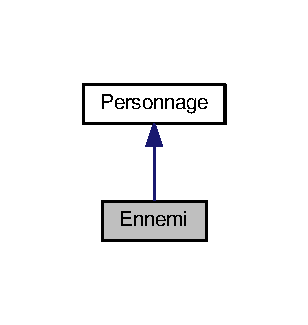
\includegraphics[width=148pt]{classEnnemi__inherit__graph}
\end{center}
\end{figure}


Graphe de collaboration de Ennemi\+:
\nopagebreak
\begin{figure}[H]
\begin{center}
\leavevmode
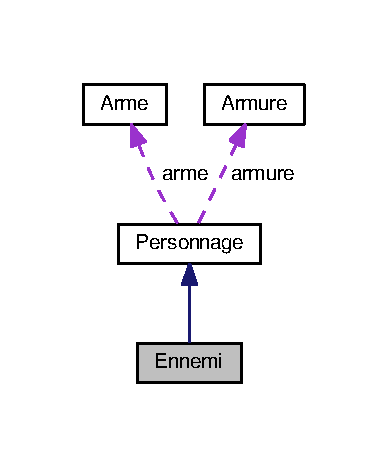
\includegraphics[width=148pt]{classEnnemi__coll__graph}
\end{center}
\end{figure}
\subsection*{Fonctions membres publiques}
\begin{DoxyCompactItemize}
\item 
\hyperlink{classEnnemi_a9c5eb7ca82848b97f3dcf262fe625b3a}{Ennemi} ()
\begin{DoxyCompactList}\small\item\em Classe ennemi. \end{DoxyCompactList}\item 
\hyperlink{classEnnemi_a7ada13b6147e695401fdb41126a6c07b}{Ennemi} (int position\+X, int position\+Y, Arme arme, Armure armure, clan\+::\+Image sprite)
\end{DoxyCompactItemize}
\subsection*{Membres hérités additionnels}


\subsection{Documentation des constructeurs et destructeur}
\hypertarget{classEnnemi_a9c5eb7ca82848b97f3dcf262fe625b3a}{}\index{Ennemi@{Ennemi}!Ennemi@{Ennemi}}
\index{Ennemi@{Ennemi}!Ennemi@{Ennemi}}
\subsubsection[{Ennemi}]{\setlength{\rightskip}{0pt plus 5cm}Ennemi\+::\+Ennemi (
\begin{DoxyParamCaption}
{}
\end{DoxyParamCaption}
)}\label{classEnnemi_a9c5eb7ca82848b97f3dcf262fe625b3a}


Classe ennemi. 

Implémentation de la classe \hyperlink{classEnnemi}{Ennemi} et de ses méthodes; \begin{DoxyAuthor}{Auteur}
Geoffrey D\+E\+S\+B\+R\+O\+S\+S\+E\+S 
\end{DoxyAuthor}
\begin{DoxyVersion}{Version}
1 
\end{DoxyVersion}
\begin{DoxyDate}{Date}
2015-\/12-\/09
\end{DoxyDate}
Constructeur de l\textquotesingle{}ennemi. \begin{DoxyReturn}{Renvoie}
\hyperlink{classEnnemi}{Ennemi} l\textquotesingle{}ennemi créé. 
\end{DoxyReturn}
\hypertarget{classEnnemi_a7ada13b6147e695401fdb41126a6c07b}{}\index{Ennemi@{Ennemi}!Ennemi@{Ennemi}}
\index{Ennemi@{Ennemi}!Ennemi@{Ennemi}}
\subsubsection[{Ennemi}]{\setlength{\rightskip}{0pt plus 5cm}Ennemi\+::\+Ennemi (
\begin{DoxyParamCaption}
\item[{int}]{x, }
\item[{int}]{y, }
\item[{Arme}]{arme, }
\item[{Armure}]{armure, }
\item[{clan\+::\+Image}]{sprite}
\end{DoxyParamCaption}
)}\label{classEnnemi_a7ada13b6147e695401fdb41126a6c07b}
Constructeur de l\textquotesingle{}ennemi. 
\begin{DoxyParams}[1]{Paramètres}
\mbox{\tt in}  & {\em x} & la position en x de l\textquotesingle{}ennemi à créer. \\
\hline
\mbox{\tt in}  & {\em y} & la position en y de l\textquotesingle{}ennemi à créer. \\
\hline
\mbox{\tt in}  & {\em arme} & L\textquotesingle{}arme de l\textquotesingle{}ennemi. \\
\hline
\mbox{\tt in}  & {\em armure} & L\textquotesingle{}armure de l\textquotesingle{}ennemi. \\
\hline
\mbox{\tt in}  & {\em sprite} & L\textquotesingle{}image de l\textquotesingle{}ennemi. \\
\hline
\end{DoxyParams}
\begin{DoxyReturn}{Renvoie}
\hyperlink{classEnnemi}{Ennemi} l\textquotesingle{}ennemi créé. 
\end{DoxyReturn}


La documentation de cette classe a été générée à partir des fichiers suivants \+:\begin{DoxyCompactItemize}
\item 
Code\+Main/ennemi.\+hpp\item 
Code\+Main/ennemi.\+cpp\end{DoxyCompactItemize}

\hypertarget{classMap}{}\section{Référence de la classe Map}
\label{classMap}\index{Map@{Map}}
\subsection*{Fonctions membres publiques}
\begin{DoxyCompactItemize}
\item 
\hyperlink{classMap_a0f5ad0fd4563497b4214038cbca8b582}{Map} ()
\begin{DoxyCompactList}\small\item\em Construit et dessine une carte. \end{DoxyCompactList}\item 
\hyperlink{classMap_a46ac1f99aad9f30fe227bbcbbc9bfb40}{Map} (int height, int width, \hyperlink{classTileset}{Tileset} tileset)
\item 
\hyperlink{classMap_a2cd2cd94fc4acf3d4929fb657ea2708f}{Map} (std\+::string tmx\+File, \hyperlink{classTileset}{Tileset} tileset)
\item 
\hyperlink{classMap_ad656e50a9b15ff4eb04c1b603d11d0f3}{Map} (const \hyperlink{classMap}{Map} \&orig)
\item 
virtual \hyperlink{classMap_aa403fbe09394ccf39747588f5168e3b2}{$\sim$\+Map} ()
\item 
int \hyperlink{classMap_a2b09c8875af2efb711fc3a022e70427d}{get\+Height} ()
\item 
int \hyperlink{classMap_afd34d12227676b3cebeed9f5fae2508f}{get\+Width} ()
\item 
vector$<$ vector$<$ int $>$ $>$ \hyperlink{classMap_a06f3a536bfac5e0e23497aa7b3bff0eb}{get\+Tiles} ()
\item 
int \hyperlink{classMap_addae7f55daf2a95b893bbeb4807fa7ec}{get\+Tile\+At} (int x, int y)
\item 
void \hyperlink{classMap_ac7894d7c53218b8a323119ed7cd9969a}{set\+Tile\+At} (int x, int y, int tile)
\item 
int \hyperlink{classMap_a1a165f12a747bc248016964acabfbc0e}{get\+Tile\+Size} ()
\item 
vector$<$ vector$<$ int $>$ $>$ \hyperlink{classMap_a0a937e8ca98865f0fff39657b70fc6fe}{get\+Collision\+Map} ()
\item 
void \hyperlink{classMap_ae7fb26d285fa138b674394b59d5186d9}{set\+Collision\+Map} (vector$<$ int $>$ passable\+\_\+tiles)
\item 
void \hyperlink{classMap_aa7b78361476169633bb9236ab2300381}{read\+Tmx\+File} (std\+::string file)
\item 
void \hyperlink{classMap_aa92361fe9347de4548b31a306f77764e}{draw\+Map} (clan\+::\+Canvas c)
\item 
void \hyperlink{classMap_a8bd29f94b805b8e29e4eac427e2ff0e1}{draw\+Map} (clan\+::\+Canvas c, int x, int y)
\end{DoxyCompactItemize}


\subsection{Documentation des constructeurs et destructeur}
\hypertarget{classMap_a0f5ad0fd4563497b4214038cbca8b582}{}\index{Map@{Map}!Map@{Map}}
\index{Map@{Map}!Map@{Map}}
\subsubsection[{Map}]{\setlength{\rightskip}{0pt plus 5cm}Map\+::\+Map (
\begin{DoxyParamCaption}
{}
\end{DoxyParamCaption}
)}\label{classMap_a0f5ad0fd4563497b4214038cbca8b582}


Construit et dessine une carte. 

\begin{DoxyAuthor}{Auteur}
Clément Bauchet 
\end{DoxyAuthor}
\begin{DoxyVersion}{Version}
1 
\end{DoxyVersion}
\begin{DoxyDate}{Date}
20 novembre 2015, 19\+:22
\end{DoxyDate}
Constructeur de la map par défaut. \begin{DoxyReturn}{Renvoie}
la \hyperlink{classMap}{Map} créée. 
\end{DoxyReturn}
\hypertarget{classMap_a46ac1f99aad9f30fe227bbcbbc9bfb40}{}\index{Map@{Map}!Map@{Map}}
\index{Map@{Map}!Map@{Map}}
\subsubsection[{Map}]{\setlength{\rightskip}{0pt plus 5cm}Map\+::\+Map (
\begin{DoxyParamCaption}
\item[{int}]{height, }
\item[{int}]{width, }
\item[{{\bf Tileset}}]{tileset}
\end{DoxyParamCaption}
)}\label{classMap_a46ac1f99aad9f30fe227bbcbbc9bfb40}
Création d\textquotesingle{}une carte de taille donnée. 
\begin{DoxyParams}[1]{Paramètres}
\mbox{\tt in}  & {\em height} & La hauteur de la map à créer. \\
\hline
\mbox{\tt in}  & {\em width} & La largeur de la map à créer. \\
\hline
\mbox{\tt in}  & {\em tileset} & Le tileset à charger pour dessiner la map. \\
\hline
\mbox{\tt out}  & {\em height} & La hauteur de la map en cases. \\
\hline
\mbox{\tt out}  & {\em width} & La largeur de la map en cases. \\
\hline
\mbox{\tt out}  & {\em tiles} & La matrice des cases de la carte \\
\hline
\mbox{\tt out}  & {\em collision\+\_\+map} & La matrice de collision de la carte \\
\hline
\mbox{\tt out}  & {\em tileset} & Le tileset utilisé pour dessiner la map. \\
\hline
\mbox{\tt out}  & {\em tile\+\_\+size} & la taille en pixels des cases du tileset utilisé (en supposant les tiles carrés). \\
\hline
\end{DoxyParams}
\begin{DoxyReturn}{Renvoie}
la \hyperlink{classMap}{Map} créée. 
\end{DoxyReturn}
\hypertarget{classMap_a2cd2cd94fc4acf3d4929fb657ea2708f}{}\index{Map@{Map}!Map@{Map}}
\index{Map@{Map}!Map@{Map}}
\subsubsection[{Map}]{\setlength{\rightskip}{0pt plus 5cm}Map\+::\+Map (
\begin{DoxyParamCaption}
\item[{std\+::string}]{tmx\+File, }
\item[{{\bf Tileset}}]{tileset}
\end{DoxyParamCaption}
)}\label{classMap_a2cd2cd94fc4acf3d4929fb657ea2708f}
Création d\textquotesingle{}une carte à partir du seul fichier .tmx 
\begin{DoxyParams}[1]{Paramètres}
\mbox{\tt in}  & {\em tmx\+File} & le fichier au format .tmx contenant les données de la carte. \\
\hline
\mbox{\tt in}  & {\em tileset} & le tileset contenant les tiles à dessiner. \\
\hline
\mbox{\tt out}  & {\em height} & La hauteur de la map. \\
\hline
\mbox{\tt out}  & {\em width} & La largeur de la map. \\
\hline
\mbox{\tt out}  & {\em tileset} & Le tileset utilisé pour dessiner la map. \\
\hline
\mbox{\tt out}  & {\em tile\+\_\+size} & la taille en pixels des cases du tileset utilisé (en supposant les tiles carrés). \\
\hline
\mbox{\tt out}  & {\em tiles} & La matrice des cases de la carte \\
\hline
\end{DoxyParams}
\hypertarget{classMap_ad656e50a9b15ff4eb04c1b603d11d0f3}{}\index{Map@{Map}!Map@{Map}}
\index{Map@{Map}!Map@{Map}}
\subsubsection[{Map}]{\setlength{\rightskip}{0pt plus 5cm}Map\+::\+Map (
\begin{DoxyParamCaption}
\item[{const {\bf Map} \&}]{orig}
\end{DoxyParamCaption}
)}\label{classMap_ad656e50a9b15ff4eb04c1b603d11d0f3}
Création d\textquotesingle{}une carte par copie d\textquotesingle{}une autre \begin{DoxyAuthor}{Auteur}
Clément Bauchet 
\end{DoxyAuthor}

\begin{DoxyParams}[1]{Paramètres}
\mbox{\tt in}  & {\em orig} & La \hyperlink{classMap}{Map} à copier. \\
\hline
\mbox{\tt out}  & {\em height} & La hauteur de la map. \\
\hline
\mbox{\tt out}  & {\em width} & La largeur de la map. \\
\hline
\mbox{\tt out}  & {\em tiles} & La matrice des cases de la carte \\
\hline
\mbox{\tt out}  & {\em collision\+\_\+map} & La matrice de collision de la carte \\
\hline
\mbox{\tt out}  & {\em tileset} & Le tileset utilisé pour dessiner la map. \\
\hline
\mbox{\tt out}  & {\em tile\+\_\+size} & la taille en pixels des cases du tileset utilisé (en supposant les tiles carrés). \\
\hline
\end{DoxyParams}
\begin{DoxyReturn}{Renvoie}
la \hyperlink{classMap}{Map} créée. 
\end{DoxyReturn}
\hypertarget{classMap_aa403fbe09394ccf39747588f5168e3b2}{}\index{Map@{Map}!````~Map@{$\sim$\+Map}}
\index{````~Map@{$\sim$\+Map}!Map@{Map}}
\subsubsection[{$\sim$\+Map}]{\setlength{\rightskip}{0pt plus 5cm}Map\+::$\sim$\+Map (
\begin{DoxyParamCaption}
{}
\end{DoxyParamCaption}
)\hspace{0.3cm}{\ttfamily [virtual]}}\label{classMap_aa403fbe09394ccf39747588f5168e3b2}
Destructeur de la map. 

\subsection{Documentation des fonctions membres}
\hypertarget{classMap_aa92361fe9347de4548b31a306f77764e}{}\index{Map@{Map}!draw\+Map@{draw\+Map}}
\index{draw\+Map@{draw\+Map}!Map@{Map}}
\subsubsection[{draw\+Map}]{\setlength{\rightskip}{0pt plus 5cm}void Map\+::draw\+Map (
\begin{DoxyParamCaption}
\item[{clan\+::\+Canvas}]{c}
\end{DoxyParamCaption}
)}\label{classMap_aa92361fe9347de4548b31a306f77764e}
Dessine la carte dans le canvas. 
\begin{DoxyParams}[1]{Paramètres}
\mbox{\tt in}  & {\em c} & le canvas dans lequel dessiner \\
\hline
\end{DoxyParams}
\hypertarget{classMap_a8bd29f94b805b8e29e4eac427e2ff0e1}{}\index{Map@{Map}!draw\+Map@{draw\+Map}}
\index{draw\+Map@{draw\+Map}!Map@{Map}}
\subsubsection[{draw\+Map}]{\setlength{\rightskip}{0pt plus 5cm}void Map\+::draw\+Map (
\begin{DoxyParamCaption}
\item[{clan\+::\+Canvas}]{c, }
\item[{int}]{x, }
\item[{int}]{y}
\end{DoxyParamCaption}
)}\label{classMap_a8bd29f94b805b8e29e4eac427e2ff0e1}
Dessine la carte dans le canvas à une position donnée. 
\begin{DoxyParams}[1]{Paramètres}
\mbox{\tt in}  & {\em c} & Le canvas dans lequel dessiner à une certaine position. \\
\hline
\mbox{\tt in}  & {\em x} & La coordonnée x de la position du canvas où dessiner \\
\hline
\mbox{\tt in}  & {\em y} & La coordonnée y de la position du canvas où dessiner \\
\hline
\end{DoxyParams}
\hypertarget{classMap_a0a937e8ca98865f0fff39657b70fc6fe}{}\index{Map@{Map}!get\+Collision\+Map@{get\+Collision\+Map}}
\index{get\+Collision\+Map@{get\+Collision\+Map}!Map@{Map}}
\subsubsection[{get\+Collision\+Map}]{\setlength{\rightskip}{0pt plus 5cm}vector$<$ vector$<$ int $>$ $>$ Map\+::get\+Collision\+Map (
\begin{DoxyParamCaption}
{}
\end{DoxyParamCaption}
)}\label{classMap_a0a937e8ca98865f0fff39657b70fc6fe}
Méthode qui retourne la matrice de collision de la carte. 
\begin{DoxyParams}[1]{Paramètres}
\mbox{\tt out}  & {\em file} & La matrice de collision de la carte. \\
\hline
\end{DoxyParams}
\hypertarget{classMap_a2b09c8875af2efb711fc3a022e70427d}{}\index{Map@{Map}!get\+Height@{get\+Height}}
\index{get\+Height@{get\+Height}!Map@{Map}}
\subsubsection[{get\+Height}]{\setlength{\rightskip}{0pt plus 5cm}int Map\+::get\+Height (
\begin{DoxyParamCaption}
{}
\end{DoxyParamCaption}
)}\label{classMap_a2b09c8875af2efb711fc3a022e70427d}
Getter de l\textquotesingle{}attribut height. \begin{DoxyReturn}{Renvoie}
height La hauteur de la carte en cases. 
\end{DoxyReturn}
\hypertarget{classMap_addae7f55daf2a95b893bbeb4807fa7ec}{}\index{Map@{Map}!get\+Tile\+At@{get\+Tile\+At}}
\index{get\+Tile\+At@{get\+Tile\+At}!Map@{Map}}
\subsubsection[{get\+Tile\+At}]{\setlength{\rightskip}{0pt plus 5cm}int Map\+::get\+Tile\+At (
\begin{DoxyParamCaption}
\item[{int}]{row, }
\item[{int}]{col}
\end{DoxyParamCaption}
)}\label{classMap_addae7f55daf2a95b893bbeb4807fa7ec}
Getter de la valeur de la case à une position donnée. 
\begin{DoxyParams}[1]{Paramètres}
\mbox{\tt in}  & {\em row} & La ligne à laquelle se trouve la case. \\
\hline
\mbox{\tt in}  & {\em col} & La colonne à laquelel se trouve la case. \\
\hline
\end{DoxyParams}
\begin{DoxyReturn}{Renvoie}
tiles Un entier représentant le type de case présent à la position (row, col). 
\end{DoxyReturn}
\hypertarget{classMap_a06f3a536bfac5e0e23497aa7b3bff0eb}{}\index{Map@{Map}!get\+Tiles@{get\+Tiles}}
\index{get\+Tiles@{get\+Tiles}!Map@{Map}}
\subsubsection[{get\+Tiles}]{\setlength{\rightskip}{0pt plus 5cm}vector$<$ vector$<$ int $>$ $>$ Map\+::get\+Tiles (
\begin{DoxyParamCaption}
{}
\end{DoxyParamCaption}
)}\label{classMap_a06f3a536bfac5e0e23497aa7b3bff0eb}
Getter de l\textquotesingle{}attribut tiles. \begin{DoxyReturn}{Renvoie}
tiles La matrice des cases de la carte. 
\end{DoxyReturn}
\hypertarget{classMap_a1a165f12a747bc248016964acabfbc0e}{}\index{Map@{Map}!get\+Tile\+Size@{get\+Tile\+Size}}
\index{get\+Tile\+Size@{get\+Tile\+Size}!Map@{Map}}
\subsubsection[{get\+Tile\+Size}]{\setlength{\rightskip}{0pt plus 5cm}int Map\+::get\+Tile\+Size (
\begin{DoxyParamCaption}
{}
\end{DoxyParamCaption}
)}\label{classMap_a1a165f12a747bc248016964acabfbc0e}
Getter de l\textquotesingle{}attribut tile\+\_\+size. \begin{DoxyReturn}{Renvoie}
tile\+\_\+size La taille en pixels des cases (en supposant les cases carrées). 
\end{DoxyReturn}
\hypertarget{classMap_afd34d12227676b3cebeed9f5fae2508f}{}\index{Map@{Map}!get\+Width@{get\+Width}}
\index{get\+Width@{get\+Width}!Map@{Map}}
\subsubsection[{get\+Width}]{\setlength{\rightskip}{0pt plus 5cm}int Map\+::get\+Width (
\begin{DoxyParamCaption}
{}
\end{DoxyParamCaption}
)}\label{classMap_afd34d12227676b3cebeed9f5fae2508f}
Getter de l\textquotesingle{}attribut width. \begin{DoxyReturn}{Renvoie}
width La largeur de la carte en cases. 
\end{DoxyReturn}
\hypertarget{classMap_aa7b78361476169633bb9236ab2300381}{}\index{Map@{Map}!read\+Tmx\+File@{read\+Tmx\+File}}
\index{read\+Tmx\+File@{read\+Tmx\+File}!Map@{Map}}
\subsubsection[{read\+Tmx\+File}]{\setlength{\rightskip}{0pt plus 5cm}void Map\+::read\+Tmx\+File (
\begin{DoxyParamCaption}
\item[{std\+::string}]{file}
\end{DoxyParamCaption}
)}\label{classMap_aa7b78361476169633bb9236ab2300381}
Méthode qui permet de remplir la matrice de cases de la carte à partir d\textquotesingle{}un fichier X\+M\+L. 
\begin{DoxyParams}[1]{Paramètres}
\mbox{\tt in}  & {\em file} & Le nom du fichier à lire. \\
\hline
\end{DoxyParams}
\hypertarget{classMap_ae7fb26d285fa138b674394b59d5186d9}{}\index{Map@{Map}!set\+Collision\+Map@{set\+Collision\+Map}}
\index{set\+Collision\+Map@{set\+Collision\+Map}!Map@{Map}}
\subsubsection[{set\+Collision\+Map}]{\setlength{\rightskip}{0pt plus 5cm}void Map\+::set\+Collision\+Map (
\begin{DoxyParamCaption}
\item[{vector$<$ int $>$}]{passable\+\_\+tiles}
\end{DoxyParamCaption}
)}\label{classMap_ae7fb26d285fa138b674394b59d5186d9}
Méthode qui établit la matrice de collision de la carte, en fonction d\textquotesingle{}une liste d\textquotesingle{}id de cases passables. 
\begin{DoxyParams}[1]{Paramètres}
\mbox{\tt out}  & {\em file} & La matrice de collision de la carte. \\
\hline
\end{DoxyParams}
\hypertarget{classMap_ac7894d7c53218b8a323119ed7cd9969a}{}\index{Map@{Map}!set\+Tile\+At@{set\+Tile\+At}}
\index{set\+Tile\+At@{set\+Tile\+At}!Map@{Map}}
\subsubsection[{set\+Tile\+At}]{\setlength{\rightskip}{0pt plus 5cm}void Map\+::set\+Tile\+At (
\begin{DoxyParamCaption}
\item[{int}]{row, }
\item[{int}]{col, }
\item[{int}]{tile}
\end{DoxyParamCaption}
)}\label{classMap_ac7894d7c53218b8a323119ed7cd9969a}
Setter de l\textquotesingle{}attribut tiles. Modifie la case à une certaine position. 
\begin{DoxyParams}[1]{Paramètres}
\mbox{\tt in}  & {\em row} & la ligne à laquelle se trouve la case à modifier. \\
\hline
\mbox{\tt in}  & {\em col} & la colonne à laquelle se trouve la case à modifier. \\
\hline
\mbox{\tt in}  & {\em tile} & la nouvelle valeur de la case à modifier. \\
\hline
\mbox{\tt out}  & {\em tiles} & la nouvelle valeur de la case en (row, col). \\
\hline
\end{DoxyParams}


La documentation de cette classe a été générée à partir des fichiers suivants \+:\begin{DoxyCompactItemize}
\item 
Code\+Main/map.\+hpp\item 
Code\+Main/map.\+cpp\end{DoxyCompactItemize}

\hypertarget{classMapDisplay}{}\section{Référence de la classe Map\+Display}
\label{classMapDisplay}\index{Map\+Display@{Map\+Display}}


Graphe d\textquotesingle{}héritage de Map\+Display\+:
\nopagebreak
\begin{figure}[H]
\begin{center}
\leavevmode
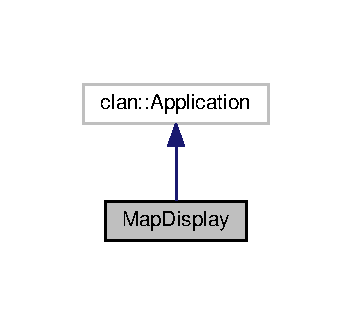
\includegraphics[width=169pt]{classMapDisplay__inherit__graph}
\end{center}
\end{figure}


Graphe de collaboration de Map\+Display\+:
\nopagebreak
\begin{figure}[H]
\begin{center}
\leavevmode
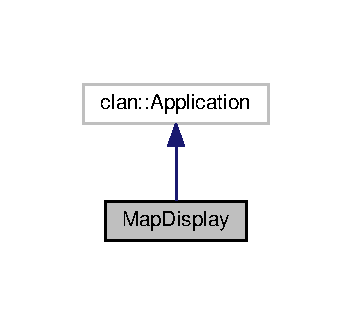
\includegraphics[width=169pt]{classMapDisplay__coll__graph}
\end{center}
\end{figure}
\subsection*{Fonctions membres publiques}
\begin{DoxyCompactItemize}
\item 
\hyperlink{classMapDisplay_a1f0a215583b172d49fa855ac9320c35a}{Map\+Display} ()
\item 
bool \hyperlink{classMapDisplay_ac3f929716c8d0451c59bda3574429ee3}{update} () override
\end{DoxyCompactItemize}


\subsection{Documentation des constructeurs et destructeur}
\hypertarget{classMapDisplay_a1f0a215583b172d49fa855ac9320c35a}{}\index{Map\+Display@{Map\+Display}!Map\+Display@{Map\+Display}}
\index{Map\+Display@{Map\+Display}!Map\+Display@{Map\+Display}}
\subsubsection[{Map\+Display}]{\setlength{\rightskip}{0pt plus 5cm}Map\+Display\+::\+Map\+Display (
\begin{DoxyParamCaption}
{}
\end{DoxyParamCaption}
)}\label{classMapDisplay_a1f0a215583b172d49fa855ac9320c35a}
Classe gérant l\textquotesingle{}affichage graphique du terrain et des éléments présents dessus. 

\subsection{Documentation des fonctions membres}
\hypertarget{classMapDisplay_ac3f929716c8d0451c59bda3574429ee3}{}\index{Map\+Display@{Map\+Display}!update@{update}}
\index{update@{update}!Map\+Display@{Map\+Display}}
\subsubsection[{update}]{\setlength{\rightskip}{0pt plus 5cm}bool Map\+Display\+::update (
\begin{DoxyParamCaption}
{}
\end{DoxyParamCaption}
)\hspace{0.3cm}{\ttfamily [override]}}\label{classMapDisplay_ac3f929716c8d0451c59bda3574429ee3}
Méthode mettant à jour l\textquotesingle{}application et redessinant tout \begin{DoxyReturn}{Renvoie}
quit un booléen indiquant si l\textquotesingle{}application doit être quittée ou non 
\end{DoxyReturn}


La documentation de cette classe a été générée à partir des fichiers suivants \+:\begin{DoxyCompactItemize}
\item 
Code\+Main/map\+Display.\+hpp\item 
Code\+Main/map\+Display.\+cpp\end{DoxyCompactItemize}

\hypertarget{classMapDisplayTestPathfinding}{}\section{Référence de la classe Map\+Display\+Test\+Pathfinding}
\label{classMapDisplayTestPathfinding}\index{Map\+Display\+Test\+Pathfinding@{Map\+Display\+Test\+Pathfinding}}


Graphe d\textquotesingle{}héritage de Map\+Display\+Test\+Pathfinding\+:\nopagebreak
\begin{figure}[H]
\begin{center}
\leavevmode
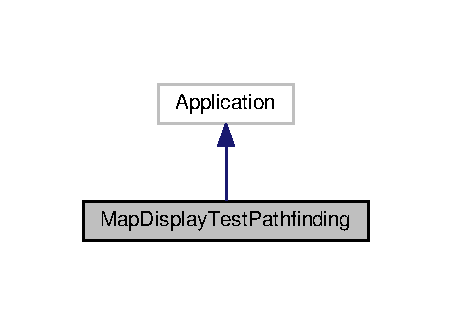
\includegraphics[width=217pt]{classMapDisplayTestPathfinding__inherit__graph}
\end{center}
\end{figure}


Graphe de collaboration de Map\+Display\+Test\+Pathfinding\+:\nopagebreak
\begin{figure}[H]
\begin{center}
\leavevmode
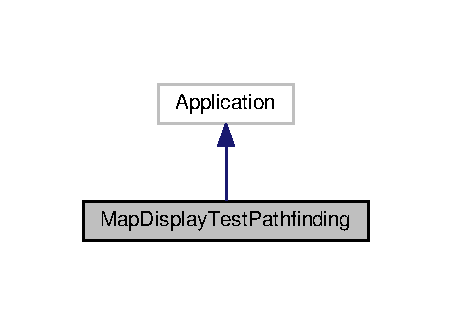
\includegraphics[width=217pt]{classMapDisplayTestPathfinding__coll__graph}
\end{center}
\end{figure}
\subsection*{Fonctions membres publiques}
\begin{DoxyCompactItemize}
\item 
\hyperlink{classMapDisplayTestPathfinding_a97c5acec6743b1099a6e6827e0b77a78}{Map\+Display\+Test\+Pathfinding} ()
\item 
bool \hyperlink{classMapDisplayTestPathfinding_a1286ccf10d21d40419ec5c900d3998f3}{update} () override
\item 
void \hyperlink{classMapDisplayTestPathfinding_acf7f5c72f302fa74bdee6702d497307b}{go\+To} (\hyperlink{classPersonnage}{Personnage} perso, std\+::string path)
\item 
void \hyperlink{classMapDisplayTestPathfinding_a544fd59caaae448044c21c8423da9a31}{exploration\+Robot} (\hyperlink{classRobot}{Robot} robot, vector$<$ \hyperlink{classClef}{Clef} $>$ liste\+\_\+clefs, vector$<$ \hyperlink{classCoffre}{Coffre} $>$ liste\+\_\+coffres)
\item 
void \hyperlink{classMapDisplayTestPathfinding_a04dc1aac567305afdd7ca99255127677}{exploration\+Ennemi} (\hyperlink{classEnnemi}{Ennemi} ennemi)
\item 
\hypertarget{classMapDisplayTestPathfinding_aea2d2a8e916ce118217a5ee0b9ff47eb}{}\hyperlink{classCoffre}{Coffre} {\bfseries find\+Nearest\+Chest} (\hyperlink{classRobot}{Robot} robot, vector$<$ \hyperlink{classCoffre}{Coffre} $>$ liste\+\_\+coffres)\label{classMapDisplayTestPathfinding_aea2d2a8e916ce118217a5ee0b9ff47eb}

\item 
\hypertarget{classMapDisplayTestPathfinding_abefa4a37705752a473e412fb2ce6112b}{}\hyperlink{classCoffre}{Coffre} {\bfseries find\+Nearest\+Key} (\hyperlink{classRobot}{Robot} robot, vector$<$ \hyperlink{classClef}{Clef} $>$ liste\+\_\+clefs)\label{classMapDisplayTestPathfinding_abefa4a37705752a473e412fb2ce6112b}

\end{DoxyCompactItemize}


\subsection{Documentation des constructeurs et destructeur}
\hypertarget{classMapDisplayTestPathfinding_a97c5acec6743b1099a6e6827e0b77a78}{}\index{Map\+Display\+Test\+Pathfinding@{Map\+Display\+Test\+Pathfinding}!Map\+Display\+Test\+Pathfinding@{Map\+Display\+Test\+Pathfinding}}
\index{Map\+Display\+Test\+Pathfinding@{Map\+Display\+Test\+Pathfinding}!Map\+Display\+Test\+Pathfinding@{Map\+Display\+Test\+Pathfinding}}
\subsubsection[{Map\+Display\+Test\+Pathfinding}]{\setlength{\rightskip}{0pt plus 5cm}Map\+Display\+Test\+Pathfinding\+::\+Map\+Display\+Test\+Pathfinding (
\begin{DoxyParamCaption}
{}
\end{DoxyParamCaption}
)}\label{classMapDisplayTestPathfinding_a97c5acec6743b1099a6e6827e0b77a78}
Classe gérant l\textquotesingle{}affichage graphique du terrain et des éléments présents dessus. 

\subsection{Documentation des fonctions membres}
\hypertarget{classMapDisplayTestPathfinding_a04dc1aac567305afdd7ca99255127677}{}\index{Map\+Display\+Test\+Pathfinding@{Map\+Display\+Test\+Pathfinding}!exploration\+Ennemi@{exploration\+Ennemi}}
\index{exploration\+Ennemi@{exploration\+Ennemi}!Map\+Display\+Test\+Pathfinding@{Map\+Display\+Test\+Pathfinding}}
\subsubsection[{exploration\+Ennemi}]{\setlength{\rightskip}{0pt plus 5cm}void Map\+Display\+Test\+Pathfinding\+::exploration\+Ennemi (
\begin{DoxyParamCaption}
\item[{{\bf Ennemi}}]{ennemi}
\end{DoxyParamCaption}
)}\label{classMapDisplayTestPathfinding_a04dc1aac567305afdd7ca99255127677}
Routine d\textquotesingle{}exploration d\textquotesingle{}un ennemi 
\begin{DoxyParams}[1]{Paramètres}
\mbox{\tt in}  & {\em ennemi} & l\textquotesingle{}ennemi qui explore la carte de façon aléatoire \\
\hline
\end{DoxyParams}
\hypertarget{classMapDisplayTestPathfinding_a544fd59caaae448044c21c8423da9a31}{}\index{Map\+Display\+Test\+Pathfinding@{Map\+Display\+Test\+Pathfinding}!exploration\+Robot@{exploration\+Robot}}
\index{exploration\+Robot@{exploration\+Robot}!Map\+Display\+Test\+Pathfinding@{Map\+Display\+Test\+Pathfinding}}
\subsubsection[{exploration\+Robot}]{\setlength{\rightskip}{0pt plus 5cm}void Map\+Display\+Test\+Pathfinding\+::exploration\+Robot (
\begin{DoxyParamCaption}
\item[{{\bf Robot}}]{robot, }
\item[{vector$<$ {\bf Clef} $>$}]{liste\+\_\+clefs, }
\item[{vector$<$ {\bf Coffre} $>$}]{liste\+\_\+coffres}
\end{DoxyParamCaption}
)}\label{classMapDisplayTestPathfinding_a544fd59caaae448044c21c8423da9a31}
Routine d\textquotesingle{}exploration du robot 
\begin{DoxyParams}[1]{Paramètres}
\mbox{\tt in}  & {\em robot,le} & robot qui explore \\
\hline
\mbox{\tt in}  & {\em liste\+\_\+clefs} & \\
\hline
\mbox{\tt in}  & {\em liste\+\_\+coffres} & \\
\hline
\end{DoxyParams}
\hypertarget{classMapDisplayTestPathfinding_acf7f5c72f302fa74bdee6702d497307b}{}\index{Map\+Display\+Test\+Pathfinding@{Map\+Display\+Test\+Pathfinding}!go\+To@{go\+To}}
\index{go\+To@{go\+To}!Map\+Display\+Test\+Pathfinding@{Map\+Display\+Test\+Pathfinding}}
\subsubsection[{go\+To}]{\setlength{\rightskip}{0pt plus 5cm}void Map\+Display\+Test\+Pathfinding\+::go\+To (
\begin{DoxyParamCaption}
\item[{{\bf Personnage}}]{perso, }
\item[{std\+::string}]{path}
\end{DoxyParamCaption}
)}\label{classMapDisplayTestPathfinding_acf7f5c72f302fa74bdee6702d497307b}
Méthode permattant à un personnage d\textquotesingle{}aller vers une direction en particulier. 
\begin{DoxyParams}[1]{Paramètres}
\mbox{\tt in}  & {\em perso} & Le personnage se déplaçant. \\
\hline
\mbox{\tt in}  & {\em path} & le chemin est modifie \\
\hline
\end{DoxyParams}
\hypertarget{classMapDisplayTestPathfinding_a1286ccf10d21d40419ec5c900d3998f3}{}\index{Map\+Display\+Test\+Pathfinding@{Map\+Display\+Test\+Pathfinding}!update@{update}}
\index{update@{update}!Map\+Display\+Test\+Pathfinding@{Map\+Display\+Test\+Pathfinding}}
\subsubsection[{update}]{\setlength{\rightskip}{0pt plus 5cm}bool Map\+Display\+Test\+Pathfinding\+::update (
\begin{DoxyParamCaption}
{}
\end{DoxyParamCaption}
)\hspace{0.3cm}{\ttfamily [override]}}\label{classMapDisplayTestPathfinding_a1286ccf10d21d40419ec5c900d3998f3}
Méthode mettant à jour l\textquotesingle{}application et redessinant tout \begin{DoxyReturn}{Renvoie}
quit un booléen indiquant si l\textquotesingle{}application doit être quittée ou non 
\end{DoxyReturn}


La documentation de cette classe a été générée à partir des fichiers suivants \+:\begin{DoxyCompactItemize}
\item 
Code\+Main/map\+Display\+Test\+Pathfinding.\+hpp\item 
Code\+Main/map\+Display\+Test\+Pathfinding.\+cpp\end{DoxyCompactItemize}

\input{classMine}
\hypertarget{classnode}{}\section{Référence de la classe node}
\label{classnode}\index{node@{node}}
\subsection*{Fonctions membres publiques}
\begin{DoxyCompactItemize}
\item 
\hyperlink{classnode_a82669b7358b50bd8d7888d7df4ff8dfa}{node} ()
\item 
\hypertarget{classnode_a54d5a4fd2b5bff5b796318ff4d8fa9f1}{}{\bfseries node} (int xp, int yp, int l, int p)\label{classnode_a54d5a4fd2b5bff5b796318ff4d8fa9f1}

\item 
int \hyperlink{classnode_a419596f9858640ee6d04b69b616b7cd2}{getx\+Pos} () const 
\item 
int \hyperlink{classnode_a3b5d135d5e5eac9211a9478ea9803ae7}{gety\+Pos} () const 
\item 
int \hyperlink{classnode_a78c66d7badca074b6b34ec7eca4ab106}{get\+Level} () const 
\item 
int \hyperlink{classnode_afebf5ef7f94fa7554890f03e97686de7}{get\+Priority} () const 
\item 
void \hyperlink{classnode_ad51b92de008bd5107a7b55cc61fc497b}{update\+Priority} (const int \&x\+Dest, const int \&y\+Dest)
\item 
\hypertarget{classnode_a04a186013c42fb942b6da90d2e98d4ed}{}void {\bfseries next\+Level} (const int \&i)\label{classnode_a04a186013c42fb942b6da90d2e98d4ed}

\item 
const int \& \hyperlink{classnode_a311569dff2e77c4c7953107333960a5d}{estimate} (const int \&x\+Dest, const int \&y\+Dest) const 
\end{DoxyCompactItemize}


\subsection{Documentation des constructeurs et destructeur}
\hypertarget{classnode_a82669b7358b50bd8d7888d7df4ff8dfa}{}\index{node@{node}!node@{node}}
\index{node@{node}!node@{node}}
\subsubsection[{node}]{\setlength{\rightskip}{0pt plus 5cm}node\+::node (
\begin{DoxyParamCaption}
{}
\end{DoxyParamCaption}
)}\label{classnode_a82669b7358b50bd8d7888d7df4ff8dfa}
Constructeur d\textquotesingle{}un objet node, utilisé pour calculer le chemin 
\begin{DoxyParams}[1]{Paramètres}
\mbox{\tt in}  & {\em xp} & valeur à donner à x\+Pos \\
\hline
\mbox{\tt in}  & {\em yp} & valeur à donner à y\+Pos \\
\hline
\mbox{\tt in}  & {\em l} & valeur à donner à level \\
\hline
\mbox{\tt in}  & {\em p} & valeur à donner à priorite \\
\hline
\mbox{\tt out}  & {\em x\+Pos} & position actuelle en abscisse \\
\hline
\mbox{\tt out}  & {\em y\+Pos} & position actuelle en ordonnée \\
\hline
\mbox{\tt out}  & {\em level} & valeur contenant la distance parcourue pour arriver ici \\
\hline
\mbox{\tt out}  & {\em priority} & distance déjà parcourue plus estimation de la distance restante, plus la valeur est faible plus la priorité est grande \\
\hline
\end{DoxyParams}


\subsection{Documentation des fonctions membres}
\hypertarget{classnode_a311569dff2e77c4c7953107333960a5d}{}\index{node@{node}!estimate@{estimate}}
\index{estimate@{estimate}!node@{node}}
\subsubsection[{estimate}]{\setlength{\rightskip}{0pt plus 5cm}const int \& node\+::estimate (
\begin{DoxyParamCaption}
\item[{const int \&}]{x\+Dest, }
\item[{const int \&}]{y\+Dest}
\end{DoxyParamCaption}
) const}\label{classnode_a311569dff2e77c4c7953107333960a5d}
Méthode estimant la distance restante avant l\textquotesingle{}arrivée en calculant la distance euclidienne 
\begin{DoxyParams}[1]{Paramètres}
\mbox{\tt in}  & {\em x\+Dest} & La coordonnée en abscisse du point d\textquotesingle{}arrivée \\
\hline
\mbox{\tt in}  & {\em y\+Dest} & La coordonnée en ordonnée du point d\textquotesingle{}arrivée \\
\hline
\end{DoxyParams}
\begin{DoxyReturn}{Renvoie}
dist la distance calculée 
\end{DoxyReturn}
\hypertarget{classnode_a78c66d7badca074b6b34ec7eca4ab106}{}\index{node@{node}!get\+Level@{get\+Level}}
\index{get\+Level@{get\+Level}!node@{node}}
\subsubsection[{get\+Level}]{\setlength{\rightskip}{0pt plus 5cm}int node\+::get\+Level (
\begin{DoxyParamCaption}
{}
\end{DoxyParamCaption}
) const}\label{classnode_a78c66d7badca074b6b34ec7eca4ab106}
Getter pour obtenir la distance déjà parcourue 
\begin{DoxyParams}[1]{Paramètres}
\mbox{\tt in}  & {\em aucun} & \\
\hline
\end{DoxyParams}
\begin{DoxyReturn}{Renvoie}
level 
\end{DoxyReturn}
\hypertarget{classnode_afebf5ef7f94fa7554890f03e97686de7}{}\index{node@{node}!get\+Priority@{get\+Priority}}
\index{get\+Priority@{get\+Priority}!node@{node}}
\subsubsection[{get\+Priority}]{\setlength{\rightskip}{0pt plus 5cm}int node\+::get\+Priority (
\begin{DoxyParamCaption}
{}
\end{DoxyParamCaption}
) const}\label{classnode_afebf5ef7f94fa7554890f03e97686de7}
Getter pour obtenir la priorite du node 
\begin{DoxyParams}[1]{Paramètres}
\mbox{\tt in}  & {\em aucun} & \\
\hline
\end{DoxyParams}
\begin{DoxyReturn}{Renvoie}
priority 
\end{DoxyReturn}
\hypertarget{classnode_a419596f9858640ee6d04b69b616b7cd2}{}\index{node@{node}!getx\+Pos@{getx\+Pos}}
\index{getx\+Pos@{getx\+Pos}!node@{node}}
\subsubsection[{getx\+Pos}]{\setlength{\rightskip}{0pt plus 5cm}int node\+::getx\+Pos (
\begin{DoxyParamCaption}
{}
\end{DoxyParamCaption}
) const}\label{classnode_a419596f9858640ee6d04b69b616b7cd2}
Getter pour obtenir la position en x 
\begin{DoxyParams}[1]{Paramètres}
\mbox{\tt in}  & {\em aucun} & \\
\hline
\end{DoxyParams}
\begin{DoxyReturn}{Renvoie}
x\+Pos 
\end{DoxyReturn}
\hypertarget{classnode_a3b5d135d5e5eac9211a9478ea9803ae7}{}\index{node@{node}!gety\+Pos@{gety\+Pos}}
\index{gety\+Pos@{gety\+Pos}!node@{node}}
\subsubsection[{gety\+Pos}]{\setlength{\rightskip}{0pt plus 5cm}int node\+::gety\+Pos (
\begin{DoxyParamCaption}
{}
\end{DoxyParamCaption}
) const}\label{classnode_a3b5d135d5e5eac9211a9478ea9803ae7}
Getter pour obtenir la position en y 
\begin{DoxyParams}[1]{Paramètres}
\mbox{\tt in}  & {\em aucun} & \\
\hline
\end{DoxyParams}
\begin{DoxyReturn}{Renvoie}
y\+Pos 
\end{DoxyReturn}
\hypertarget{classnode_ad51b92de008bd5107a7b55cc61fc497b}{}\index{node@{node}!update\+Priority@{update\+Priority}}
\index{update\+Priority@{update\+Priority}!node@{node}}
\subsubsection[{update\+Priority}]{\setlength{\rightskip}{0pt plus 5cm}void node\+::update\+Priority (
\begin{DoxyParamCaption}
\item[{const int \&}]{x\+Dest, }
\item[{const int \&}]{y\+Dest}
\end{DoxyParamCaption}
)}\label{classnode_ad51b92de008bd5107a7b55cc61fc497b}
Méthode mettant à jour la priorité d\textquotesingle{}un node 
\begin{DoxyParams}[1]{Paramètres}
\mbox{\tt in}  & {\em x\+Dest} & La coordonnée en abscisse du point d\textquotesingle{}arrivée \\
\hline
\mbox{\tt in}  & {\em y\+Dest} & La coordonnée en ordonnée du point d\textquotesingle{}arrivée \\
\hline
\mbox{\tt out}  & {\em priority} & mis à jour en utilisant l\textquotesingle{}estimation \\
\hline
\end{DoxyParams}


La documentation de cette classe a été générée à partir des fichiers suivants \+:\begin{DoxyCompactItemize}
\item 
Code\+Main/astar.\+hpp\item 
Code\+Main/astar.\+cpp\end{DoxyCompactItemize}

\hypertarget{classPersonnage}{}\section{Référence de la classe Personnage}
\label{classPersonnage}\index{Personnage@{Personnage}}


Graphe d\textquotesingle{}héritage de Personnage\+:\nopagebreak
\begin{figure}[H]
\begin{center}
\leavevmode
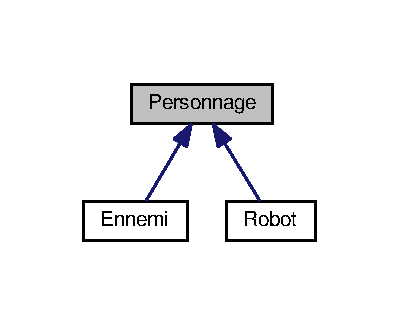
\includegraphics[width=192pt]{classPersonnage__inherit__graph}
\end{center}
\end{figure}


Graphe de collaboration de Personnage\+:
\nopagebreak
\begin{figure}[H]
\begin{center}
\leavevmode
\includegraphics[width=186pt]{classPersonnage__coll__graph}
\end{center}
\end{figure}
\subsection*{Fonctions membres publiques}
\begin{DoxyCompactItemize}
\item 
\hyperlink{classPersonnage_abec36eb0310adc71f3375297fc590c65}{Personnage} ()
\item 
\hyperlink{classPersonnage_a35385ac425d6818de9dec2d8128004a8}{Personnage} (int position\+X, int position\+Y, \hyperlink{classArme}{Arme} arme, \hyperlink{classArmure}{Armure} armure, clan\+::\+Image sprite)
\item 
int \hyperlink{classPersonnage_ab398b805fa9060fc10b5edb00685bbbb}{get\+Position\+X} ()
\item 
int \hyperlink{classPersonnage_ab19dcfb269109b0bc74ffe0143a8cda1}{get\+Position\+Y} ()
\item 
int \hyperlink{classPersonnage_ac46ff9c905454f0e3b71097b8f75c5ea}{get\+Puissance} ()
\item 
int \hyperlink{classPersonnage_a80ff0a5dc97749f73b84dd52a4185aa4}{get\+Robustesse} ()
\item 
\hyperlink{classArme}{Arme} \hyperlink{classPersonnage_a5af967c395cfccb901fb44123c373dfa}{get\+Arme} ()
\item 
\hyperlink{classArmure}{Armure} \hyperlink{classPersonnage_af0ef6f5bf22b2b471efefbd588bf4dd6}{get\+Armure} ()
\item 
void \hyperlink{classPersonnage_ae065b66e67f3a6c5781453a156786d67}{set\+Position\+X} (int x)
\item 
void \hyperlink{classPersonnage_a757454177b4a3bff5fc641ed53824154}{set\+Position\+Y} (int y)
\item 
void \hyperlink{classPersonnage_a21ee83fd23bf612ff4fadc513c78dc94}{set\+Puissance} (int puissance)
\item 
void \hyperlink{classPersonnage_a777c12bd052992cc9ccbf1f6317433c7}{set\+Robustesse} (int robustesse)
\item 
void \hyperlink{classPersonnage_a332229cbb1b8e46808472c48e7c1f3f2}{set\+Collision\+Map} (vector$<$ vector$<$ int $>$ $>$ map)
\item 
\hypertarget{classPersonnage_ab5b419f5228f8d31de209b0245ad0d64}{}vector$<$ vector$<$ int $>$ $>$ {\bfseries get\+Collision\+Map} ()\label{classPersonnage_ab5b419f5228f8d31de209b0245ad0d64}

\item 
void \hyperlink{classPersonnage_a20b675cc63e94015ddced4e7db6d9b56}{set\+Arme} (\hyperlink{classArme}{Arme} arme)
\item 
void \hyperlink{classPersonnage_a331e0aeb7190a266cfb879acdd22e83a}{set\+Armure} (\hyperlink{classArmure}{Armure} armure)
\item 
void \hyperlink{classPersonnage_afc55c03d855c3f6caf71cdb061829a6d}{deplacer} (int x, int y)
\item 
bool \hyperlink{classPersonnage_ab3b895b1830c07d547a36f0827ec9eb4}{Combattre} (\hyperlink{classPersonnage}{Personnage} $\ast$adversaire)
\item 
void \hyperlink{classPersonnage_a745bf0265378d340d7dd6f2a8225421f}{draw} (clan\+::\+Canvas c, int x, int y)
\item 
void \hyperlink{classPersonnage_ab3ce2fb4d37fc9b3bbef43d33910ac2f}{set\+Active} (bool active)
\item 
bool \hyperlink{classPersonnage_a5a95a7603154e30550bd67cf4bd4f990}{get\+Is\+Active} ()
\end{DoxyCompactItemize}
\subsection*{Attributs protégés}
\begin{DoxyCompactItemize}
\item 
\hypertarget{classPersonnage_af599fcbd1767fbf8ef5d1c90a8eaa638}{}int {\bfseries position\+X}\label{classPersonnage_af599fcbd1767fbf8ef5d1c90a8eaa638}

\item 
\hypertarget{classPersonnage_a02842b34a8c93f54772242e40e4c5a8a}{}int {\bfseries position\+Y}\label{classPersonnage_a02842b34a8c93f54772242e40e4c5a8a}

\item 
\hypertarget{classPersonnage_ac53717e24a91a7698955d506c092d2b7}{}int {\bfseries puissance}\label{classPersonnage_ac53717e24a91a7698955d506c092d2b7}

\item 
\hypertarget{classPersonnage_ab3287f35ae3106f42eb195cc60371dae}{}int {\bfseries robustesse}\label{classPersonnage_ab3287f35ae3106f42eb195cc60371dae}

\item 
\hypertarget{classPersonnage_aa724215ef4023e5444f7cdf6a6a3a8f4}{}bool {\bfseries is\+Active}\label{classPersonnage_aa724215ef4023e5444f7cdf6a6a3a8f4}

\item 
\hypertarget{classPersonnage_adf517de2c6d5f39fde55136bf8a031ea}{}clan\+::\+Image {\bfseries sprite}\label{classPersonnage_adf517de2c6d5f39fde55136bf8a031ea}

\item 
\hypertarget{classPersonnage_a5ab0e54e773a08c5efb042dfcbab9251}{}vector$<$ vector$<$ int $>$ $>$ {\bfseries collision\+\_\+map}\label{classPersonnage_a5ab0e54e773a08c5efb042dfcbab9251}

\item 
\hypertarget{classPersonnage_a538199d18a1705e6511c5f17013efd16}{}\hyperlink{classArme}{Arme} {\bfseries arme}\label{classPersonnage_a538199d18a1705e6511c5f17013efd16}

\item 
\hypertarget{classPersonnage_a0b1b3eaed5cd4f3721b22645db7833de}{}\hyperlink{classArmure}{Armure} {\bfseries armure}\label{classPersonnage_a0b1b3eaed5cd4f3721b22645db7833de}

\end{DoxyCompactItemize}


\subsection{Documentation des constructeurs et destructeur}
\hypertarget{classPersonnage_abec36eb0310adc71f3375297fc590c65}{}\index{Personnage@{Personnage}!Personnage@{Personnage}}
\index{Personnage@{Personnage}!Personnage@{Personnage}}
\subsubsection[{Personnage}]{\setlength{\rightskip}{0pt plus 5cm}Personnage\+::\+Personnage (
\begin{DoxyParamCaption}
{}
\end{DoxyParamCaption}
)}\label{classPersonnage_abec36eb0310adc71f3375297fc590c65}
Le constructeur d\textquotesingle{}un personnage par défaut. 
\begin{DoxyParams}[1]{Paramètres}
\mbox{\tt out}  & {\em is\+Active} & true par défaut pour que le personnage soit actif. \\
\hline
\end{DoxyParams}
\begin{DoxyReturn}{Renvoie}
\hyperlink{classPersonnage}{Personnage} le personnage créé. 
\end{DoxyReturn}
\hypertarget{classPersonnage_a35385ac425d6818de9dec2d8128004a8}{}\index{Personnage@{Personnage}!Personnage@{Personnage}}
\index{Personnage@{Personnage}!Personnage@{Personnage}}
\subsubsection[{Personnage}]{\setlength{\rightskip}{0pt plus 5cm}Personnage\+::\+Personnage (
\begin{DoxyParamCaption}
\item[{int}]{x, }
\item[{int}]{y, }
\item[{{\bf Arme}}]{arme, }
\item[{{\bf Armure}}]{armure, }
\item[{clan\+::\+Image}]{sprite}
\end{DoxyParamCaption}
)}\label{classPersonnage_a35385ac425d6818de9dec2d8128004a8}
Constructeur d\textquotesingle{}un personnage. 
\begin{DoxyParams}[1]{Paramètres}
\mbox{\tt in}  & {\em x} & la position en x où le personnage sera créé. \\
\hline
\mbox{\tt in}  & {\em y} & la position en y où le personnage sera créé. \\
\hline
\mbox{\tt in}  & {\em arme} & L\textquotesingle{}arme que possède le personnage. \\
\hline
\mbox{\tt in}  & {\em armure} & L\textquotesingle{}armure que possède le personnage. \\
\hline
\mbox{\tt in}  & {\em sprite} & L\textquotesingle{}image du personnage. \\
\hline
\mbox{\tt out}  & {\em position\+X} & la position en x du personnage sur la map. \\
\hline
\mbox{\tt out}  & {\em position\+Y} & la position en y du personnage sur la map. \\
\hline
\mbox{\tt out}  & {\em arme} & l\textquotesingle{}arme du personnage. \\
\hline
\mbox{\tt out}  & {\em armure} & l\textquotesingle{}armure du personnage. \\
\hline
\mbox{\tt out}  & {\em puissance} & La puissance du personnage, calculée à partir de son arme. \\
\hline
\mbox{\tt out}  & {\em robustesse} & La robustesse du personnage, calculée à partir de son armure. \\
\hline
\mbox{\tt out}  & {\em sprite} & L\textquotesingle{}image du personnage. \\
\hline
\mbox{\tt out}  & {\em is\+Active} & true par défaut pour que le personnage soit actif. \\
\hline
\end{DoxyParams}
\begin{DoxyReturn}{Renvoie}
\hyperlink{classPersonnage}{Personnage} le personnage créé. 
\end{DoxyReturn}


\subsection{Documentation des fonctions membres}
\hypertarget{classPersonnage_ab3b895b1830c07d547a36f0827ec9eb4}{}\index{Personnage@{Personnage}!Combattre@{Combattre}}
\index{Combattre@{Combattre}!Personnage@{Personnage}}
\subsubsection[{Combattre}]{\setlength{\rightskip}{0pt plus 5cm}bool Personnage\+::\+Combattre (
\begin{DoxyParamCaption}
\item[{{\bf Personnage} $\ast$}]{adversaire}
\end{DoxyParamCaption}
)}\label{classPersonnage_ab3b895b1830c07d547a36f0827ec9eb4}
Methode servant a faire affronter deux personnages du jeu. Calcul aléatoirement la force des deux adversaires et compare ces deux forces à partir de leur puissance et de leur robustesse. 
\begin{DoxyParams}[1]{Paramètres}
\mbox{\tt in}  & {\em adversaire} & Le personnage a combattre. \\
\hline
\end{DoxyParams}
\begin{DoxyReturn}{Renvoie}
victoire true si le combat est gagné, false sinon. 
\end{DoxyReturn}
\hypertarget{classPersonnage_afc55c03d855c3f6caf71cdb061829a6d}{}\index{Personnage@{Personnage}!deplacer@{deplacer}}
\index{deplacer@{deplacer}!Personnage@{Personnage}}
\subsubsection[{deplacer}]{\setlength{\rightskip}{0pt plus 5cm}void Personnage\+::deplacer (
\begin{DoxyParamCaption}
\item[{int}]{x, }
\item[{int}]{y}
\end{DoxyParamCaption}
)}\label{classPersonnage_afc55c03d855c3f6caf71cdb061829a6d}
Deplace le personnage d\textquotesingle{}une case a droite, gauche, haut ou bas. 
\begin{DoxyParams}[1]{Paramètres}
\mbox{\tt in}  & {\em x} & la valeur de déplacement en x. \\
\hline
\mbox{\tt in}  & {\em y} & la valeur de déplacement en y. \\
\hline
\mbox{\tt out}  & {\em x} & la position du personnage en x après le déplacement. \\
\hline
\mbox{\tt out}  & {\em y} & la position du personnage en y après le déplacement. \\
\hline
\end{DoxyParams}

\begin{DoxyExceptions}{Exceptions}
{\em si} & x et y en entrée ne sont pas entre -\/1 et 1. \\
\hline
{\em s\textquotesingle{}il} & n\textquotesingle{}y a aucun déplacement. \\
\hline
{\em si} & x et y sont différents de 0. \\
\hline
\end{DoxyExceptions}
\begin{DoxyReturn}{Renvoie}
rien 
\end{DoxyReturn}
\hypertarget{classPersonnage_a745bf0265378d340d7dd6f2a8225421f}{}\index{Personnage@{Personnage}!draw@{draw}}
\index{draw@{draw}!Personnage@{Personnage}}
\subsubsection[{draw}]{\setlength{\rightskip}{0pt plus 5cm}void Personnage\+::draw (
\begin{DoxyParamCaption}
\item[{clan\+::\+Canvas}]{c, }
\item[{int}]{x, }
\item[{int}]{y}
\end{DoxyParamCaption}
)}\label{classPersonnage_a745bf0265378d340d7dd6f2a8225421f}
Desinne un personnage sur la map. 
\begin{DoxyParams}[1]{Paramètres}
\mbox{\tt in}  & {\em c} & L\textquotesingle{}image du personnage. \\
\hline
\mbox{\tt in}  & {\em x} & la position en x où dessiner le personnage. \\
\hline
\mbox{\tt in}  & {\em y} & la position en y où dessiner le personnage. \\
\hline
\mbox{\tt out}  & {\em sprite} & l\textquotesingle{}image dessinée. \\
\hline
\end{DoxyParams}
\hypertarget{classPersonnage_a5af967c395cfccb901fb44123c373dfa}{}\index{Personnage@{Personnage}!get\+Arme@{get\+Arme}}
\index{get\+Arme@{get\+Arme}!Personnage@{Personnage}}
\subsubsection[{get\+Arme}]{\setlength{\rightskip}{0pt plus 5cm}{\bf Arme} Personnage\+::get\+Arme (
\begin{DoxyParamCaption}
{}
\end{DoxyParamCaption}
)}\label{classPersonnage_a5af967c395cfccb901fb44123c373dfa}
Le getter de l\textquotesingle{}arme du personnage. \begin{DoxyReturn}{Renvoie}
l\textquotesingle{}arme du personnage. 
\end{DoxyReturn}
\hypertarget{classPersonnage_af0ef6f5bf22b2b471efefbd588bf4dd6}{}\index{Personnage@{Personnage}!get\+Armure@{get\+Armure}}
\index{get\+Armure@{get\+Armure}!Personnage@{Personnage}}
\subsubsection[{get\+Armure}]{\setlength{\rightskip}{0pt plus 5cm}{\bf Armure} Personnage\+::get\+Armure (
\begin{DoxyParamCaption}
{}
\end{DoxyParamCaption}
)}\label{classPersonnage_af0ef6f5bf22b2b471efefbd588bf4dd6}
Le getter de l\textquotesingle{}armure du personnage. \begin{DoxyReturn}{Renvoie}
l\textquotesingle{}armure du personnage. 
\end{DoxyReturn}
\hypertarget{classPersonnage_a5a95a7603154e30550bd67cf4bd4f990}{}\index{Personnage@{Personnage}!get\+Is\+Active@{get\+Is\+Active}}
\index{get\+Is\+Active@{get\+Is\+Active}!Personnage@{Personnage}}
\subsubsection[{get\+Is\+Active}]{\setlength{\rightskip}{0pt plus 5cm}bool Personnage\+::get\+Is\+Active (
\begin{DoxyParamCaption}
{}
\end{DoxyParamCaption}
)}\label{classPersonnage_a5a95a7603154e30550bd67cf4bd4f990}
Getter de l\textquotesingle{}attribut is\+Activre d\textquotesingle{}un personnage. \begin{DoxyReturn}{Renvoie}
si le personnage est actif ou non. 
\end{DoxyReturn}
\hypertarget{classPersonnage_ab398b805fa9060fc10b5edb00685bbbb}{}\index{Personnage@{Personnage}!get\+Position\+X@{get\+Position\+X}}
\index{get\+Position\+X@{get\+Position\+X}!Personnage@{Personnage}}
\subsubsection[{get\+Position\+X}]{\setlength{\rightskip}{0pt plus 5cm}int Personnage\+::get\+Position\+X (
\begin{DoxyParamCaption}
{}
\end{DoxyParamCaption}
)}\label{classPersonnage_ab398b805fa9060fc10b5edb00685bbbb}
Le getter de la position en x du personnage. \begin{DoxyReturn}{Renvoie}
la position courante du personnage en x. 
\end{DoxyReturn}
\hypertarget{classPersonnage_ab19dcfb269109b0bc74ffe0143a8cda1}{}\index{Personnage@{Personnage}!get\+Position\+Y@{get\+Position\+Y}}
\index{get\+Position\+Y@{get\+Position\+Y}!Personnage@{Personnage}}
\subsubsection[{get\+Position\+Y}]{\setlength{\rightskip}{0pt plus 5cm}int Personnage\+::get\+Position\+Y (
\begin{DoxyParamCaption}
{}
\end{DoxyParamCaption}
)}\label{classPersonnage_ab19dcfb269109b0bc74ffe0143a8cda1}
Le getter de la position en y du personnage. \begin{DoxyReturn}{Renvoie}
la position courante du personnage en y. 
\end{DoxyReturn}
\hypertarget{classPersonnage_ac46ff9c905454f0e3b71097b8f75c5ea}{}\index{Personnage@{Personnage}!get\+Puissance@{get\+Puissance}}
\index{get\+Puissance@{get\+Puissance}!Personnage@{Personnage}}
\subsubsection[{get\+Puissance}]{\setlength{\rightskip}{0pt plus 5cm}int Personnage\+::get\+Puissance (
\begin{DoxyParamCaption}
{}
\end{DoxyParamCaption}
)}\label{classPersonnage_ac46ff9c905454f0e3b71097b8f75c5ea}
Le getter de la puissance du personnage. \begin{DoxyReturn}{Renvoie}
la puissance du personnage. 
\end{DoxyReturn}
\hypertarget{classPersonnage_a80ff0a5dc97749f73b84dd52a4185aa4}{}\index{Personnage@{Personnage}!get\+Robustesse@{get\+Robustesse}}
\index{get\+Robustesse@{get\+Robustesse}!Personnage@{Personnage}}
\subsubsection[{get\+Robustesse}]{\setlength{\rightskip}{0pt plus 5cm}int Personnage\+::get\+Robustesse (
\begin{DoxyParamCaption}
{}
\end{DoxyParamCaption}
)}\label{classPersonnage_a80ff0a5dc97749f73b84dd52a4185aa4}
Le getter de la robustesse du personnage. \begin{DoxyReturn}{Renvoie}
la robustesse du personnage. 
\end{DoxyReturn}
\hypertarget{classPersonnage_ab3ce2fb4d37fc9b3bbef43d33910ac2f}{}\index{Personnage@{Personnage}!set\+Active@{set\+Active}}
\index{set\+Active@{set\+Active}!Personnage@{Personnage}}
\subsubsection[{set\+Active}]{\setlength{\rightskip}{0pt plus 5cm}void Personnage\+::set\+Active (
\begin{DoxyParamCaption}
\item[{bool}]{active}
\end{DoxyParamCaption}
)}\label{classPersonnage_ab3ce2fb4d37fc9b3bbef43d33910ac2f}
passe la valeur à true de l\textquotesingle{}attribut is\+Active du personnage. 
\begin{DoxyParams}[1]{Paramètres}
\mbox{\tt out}  & {\em is\+Active} & = active. Le personnage n\textquotesingle{}est plus actif dans le jeu. \\
\hline
\end{DoxyParams}
\hypertarget{classPersonnage_a20b675cc63e94015ddced4e7db6d9b56}{}\index{Personnage@{Personnage}!set\+Arme@{set\+Arme}}
\index{set\+Arme@{set\+Arme}!Personnage@{Personnage}}
\subsubsection[{set\+Arme}]{\setlength{\rightskip}{0pt plus 5cm}void Personnage\+::set\+Arme (
\begin{DoxyParamCaption}
\item[{{\bf Arme}}]{arme}
\end{DoxyParamCaption}
)}\label{classPersonnage_a20b675cc63e94015ddced4e7db6d9b56}
Le setter de l\textquotesingle{}arme du personnage. Modifie l\textquotesingle{}arme du personnage. 
\begin{DoxyParams}[1]{Paramètres}
\mbox{\tt in}  & {\em arme} & la nouvelle arme du personnage. \\
\hline
\mbox{\tt out}  & {\em arme} & La nouvelle arme du personnage. \\
\hline
\end{DoxyParams}
\hypertarget{classPersonnage_a331e0aeb7190a266cfb879acdd22e83a}{}\index{Personnage@{Personnage}!set\+Armure@{set\+Armure}}
\index{set\+Armure@{set\+Armure}!Personnage@{Personnage}}
\subsubsection[{set\+Armure}]{\setlength{\rightskip}{0pt plus 5cm}void Personnage\+::set\+Armure (
\begin{DoxyParamCaption}
\item[{{\bf Armure}}]{armure}
\end{DoxyParamCaption}
)}\label{classPersonnage_a331e0aeb7190a266cfb879acdd22e83a}
Le setter de l\textquotesingle{}armure du personnage. Modifie l\textquotesingle{}armure du personnage. 
\begin{DoxyParams}[1]{Paramètres}
\mbox{\tt in}  & {\em armure} & la nouvelle armure du personnage. \\
\hline
\mbox{\tt out}  & {\em armure} & La nouvelle armure du personnage. \\
\hline
\end{DoxyParams}
\hypertarget{classPersonnage_a332229cbb1b8e46808472c48e7c1f3f2}{}\index{Personnage@{Personnage}!set\+Collision\+Map@{set\+Collision\+Map}}
\index{set\+Collision\+Map@{set\+Collision\+Map}!Personnage@{Personnage}}
\subsubsection[{set\+Collision\+Map}]{\setlength{\rightskip}{0pt plus 5cm}void Personnage\+::set\+Collision\+Map (
\begin{DoxyParamCaption}
\item[{vector$<$ vector$<$ int $>$ $>$}]{map}
\end{DoxyParamCaption}
)}\label{classPersonnage_a332229cbb1b8e46808472c48e7c1f3f2}
Le setter pour collision\+Map. Donne une map au personnage pour savoir là où il peut passer. 
\begin{DoxyParams}[1]{Paramètres}
\mbox{\tt in}  & {\em map} & Le vector représentant la map. \\
\hline
\mbox{\tt out}  & {\em map} & Le vector donné au personnage représentant la map courante. \\
\hline
\end{DoxyParams}
\hypertarget{classPersonnage_ae065b66e67f3a6c5781453a156786d67}{}\index{Personnage@{Personnage}!set\+Position\+X@{set\+Position\+X}}
\index{set\+Position\+X@{set\+Position\+X}!Personnage@{Personnage}}
\subsubsection[{set\+Position\+X}]{\setlength{\rightskip}{0pt plus 5cm}void Personnage\+::set\+Position\+X (
\begin{DoxyParamCaption}
\item[{int}]{x}
\end{DoxyParamCaption}
)}\label{classPersonnage_ae065b66e67f3a6c5781453a156786d67}
Le setter de la position en x du personnage. Modifie la position du personnage en x. 
\begin{DoxyParams}[1]{Paramètres}
\mbox{\tt in}  & {\em x} & la position à affecter au personnage en x. \\
\hline
\mbox{\tt out}  & {\em position\+X} & la nouvelle position en x du personnage. \\
\hline
\end{DoxyParams}
\hypertarget{classPersonnage_a757454177b4a3bff5fc641ed53824154}{}\index{Personnage@{Personnage}!set\+Position\+Y@{set\+Position\+Y}}
\index{set\+Position\+Y@{set\+Position\+Y}!Personnage@{Personnage}}
\subsubsection[{set\+Position\+Y}]{\setlength{\rightskip}{0pt plus 5cm}void Personnage\+::set\+Position\+Y (
\begin{DoxyParamCaption}
\item[{int}]{y}
\end{DoxyParamCaption}
)}\label{classPersonnage_a757454177b4a3bff5fc641ed53824154}
Le setter de la position en x du personnage. Modifie la position du personnage en y. 
\begin{DoxyParams}[1]{Paramètres}
\mbox{\tt in}  & {\em y} & la position à affecter au personnage en y. \\
\hline
\mbox{\tt out}  & {\em position\+Y} & la nouvelle position en y du personnage. \\
\hline
\end{DoxyParams}
\hypertarget{classPersonnage_a21ee83fd23bf612ff4fadc513c78dc94}{}\index{Personnage@{Personnage}!set\+Puissance@{set\+Puissance}}
\index{set\+Puissance@{set\+Puissance}!Personnage@{Personnage}}
\subsubsection[{set\+Puissance}]{\setlength{\rightskip}{0pt plus 5cm}void Personnage\+::set\+Puissance (
\begin{DoxyParamCaption}
\item[{int}]{puissance}
\end{DoxyParamCaption}
)}\label{classPersonnage_a21ee83fd23bf612ff4fadc513c78dc94}
Le setter de la puissance du personnage. Modifie la puissance du personnage. 
\begin{DoxyParams}[1]{Paramètres}
\mbox{\tt in}  & {\em puissance} & la nouvelle puissance du personnage. \\
\hline
\mbox{\tt out}  & {\em puissance} & La nouvelle puissance du personnage. \\
\hline
\end{DoxyParams}
\hypertarget{classPersonnage_a777c12bd052992cc9ccbf1f6317433c7}{}\index{Personnage@{Personnage}!set\+Robustesse@{set\+Robustesse}}
\index{set\+Robustesse@{set\+Robustesse}!Personnage@{Personnage}}
\subsubsection[{set\+Robustesse}]{\setlength{\rightskip}{0pt plus 5cm}void Personnage\+::set\+Robustesse (
\begin{DoxyParamCaption}
\item[{int}]{robustesse}
\end{DoxyParamCaption}
)}\label{classPersonnage_a777c12bd052992cc9ccbf1f6317433c7}
Le setter de la robustesse du personnage. Modifie la robustesse du personnage. 
\begin{DoxyParams}[1]{Paramètres}
\mbox{\tt in}  & {\em robustesse} & la nouvelle robustesse du personnage. \\
\hline
\mbox{\tt out}  & {\em robustesse} & La nouvelle robustesse du personnage. \\
\hline
\end{DoxyParams}


La documentation de cette classe a été générée à partir des fichiers suivants \+:\begin{DoxyCompactItemize}
\item 
Code\+Main/personnage.\+hpp\item 
Code\+Main/personnage.\+cpp\end{DoxyCompactItemize}

\hypertarget{classRobot}{}\section{Référence de la classe Robot}
\label{classRobot}\index{Robot@{Robot}}


Graphe d\textquotesingle{}héritage de Robot\+:\nopagebreak
\begin{figure}[H]
\begin{center}
\leavevmode
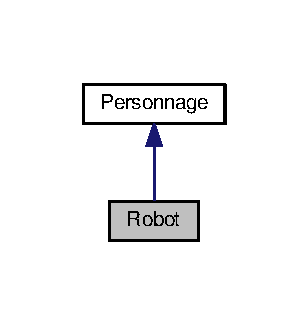
\includegraphics[width=148pt]{classRobot__inherit__graph}
\end{center}
\end{figure}


Graphe de collaboration de Robot\+:
\nopagebreak
\begin{figure}[H]
\begin{center}
\leavevmode
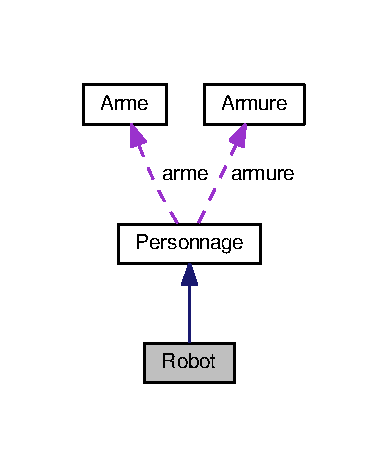
\includegraphics[width=186pt]{classRobot__coll__graph}
\end{center}
\end{figure}
\subsection*{Fonctions membres publiques}
\begin{DoxyCompactItemize}
\item 
\hyperlink{classRobot_a4fc7c70ae20623f05e06f2ecb388b6c4}{Robot} ()
\begin{DoxyCompactList}\small\item\em Classe \hyperlink{classRobot}{Robot}. \end{DoxyCompactList}\item 
\hyperlink{classRobot_a9d9ae3c384c32f3e12c4b4d294562062}{Robot} (int position\+X, int position\+Y, \hyperlink{classArme}{Arme} arme, \hyperlink{classArmure}{Armure} armure, clan\+::\+Image sprite)
\item 
int \hyperlink{classRobot_ada7c2dc3d10f11e4665ddbeaadfc2eec}{get\+Inventaire} ()
\item 
void \hyperlink{classRobot_a53f5a07f6d2adaea7703127a63af80a7}{set\+Inventaire} (int inventaire)
\item 
void \hyperlink{classRobot_a9472759b16c5988cbaa577ed37b4bb44}{ouvrir} (\hyperlink{classCoffre}{Coffre} $\ast$coffre)
\item 
void \hyperlink{classRobot_a39dd169de1eecba937e0b8fdd115c061}{ramasser} (\hyperlink{classClef}{Clef} $\ast$clef)
\end{DoxyCompactItemize}
\subsection*{Membres hérités additionnels}


\subsection{Documentation des constructeurs et destructeur}
\hypertarget{classRobot_a4fc7c70ae20623f05e06f2ecb388b6c4}{}\index{Robot@{Robot}!Robot@{Robot}}
\index{Robot@{Robot}!Robot@{Robot}}
\subsubsection[{Robot}]{\setlength{\rightskip}{0pt plus 5cm}Robot\+::\+Robot (
\begin{DoxyParamCaption}
{}
\end{DoxyParamCaption}
)}\label{classRobot_a4fc7c70ae20623f05e06f2ecb388b6c4}


Classe \hyperlink{classRobot}{Robot}. 

Implémentation de la classe \hyperlink{classRobot}{Robot} et de ses méthodes. \begin{DoxyAuthor}{Auteur}
Geoffrey D\+E\+S\+B\+R\+O\+S\+S\+E\+S 
\end{DoxyAuthor}
\begin{DoxyVersion}{Version}
1 
\end{DoxyVersion}
\begin{DoxyDate}{Date}
2015-\/12-\/09
\end{DoxyDate}
Constructeur du robot. \begin{DoxyReturn}{Renvoie}
\hyperlink{classRobot}{Robot} le robot créé. 
\end{DoxyReturn}
\hypertarget{classRobot_a9d9ae3c384c32f3e12c4b4d294562062}{}\index{Robot@{Robot}!Robot@{Robot}}
\index{Robot@{Robot}!Robot@{Robot}}
\subsubsection[{Robot}]{\setlength{\rightskip}{0pt plus 5cm}Robot\+::\+Robot (
\begin{DoxyParamCaption}
\item[{int}]{x, }
\item[{int}]{y, }
\item[{{\bf Arme}}]{arme, }
\item[{{\bf Armure}}]{armure, }
\item[{clan\+::\+Image}]{sprite}
\end{DoxyParamCaption}
)}\label{classRobot_a9d9ae3c384c32f3e12c4b4d294562062}
Constructeur du robot. 
\begin{DoxyParams}[1]{Paramètres}
\mbox{\tt in}  & {\em x} & La position en x du robot sur la carte. \\
\hline
\mbox{\tt in}  & {\em y} & La position en y du robot sur la carte. \\
\hline
\mbox{\tt in}  & {\em arme} & L\textquotesingle{}arme du robot. \\
\hline
\mbox{\tt in}  & {\em armure} & L\textquotesingle{}armure du robot. \\
\hline
\mbox{\tt in}  & {\em sprite} & L\textquotesingle{}image du robot. \\
\hline
\mbox{\tt out}  & {\em inventaire} & La taille de l\textquotesingle{}inventaire du robot, 0 par défaut. \\
\hline
\end{DoxyParams}
\begin{DoxyReturn}{Renvoie}
\hyperlink{classRobot}{Robot} le robot créé. 
\end{DoxyReturn}


\subsection{Documentation des fonctions membres}
\hypertarget{classRobot_ada7c2dc3d10f11e4665ddbeaadfc2eec}{}\index{Robot@{Robot}!get\+Inventaire@{get\+Inventaire}}
\index{get\+Inventaire@{get\+Inventaire}!Robot@{Robot}}
\subsubsection[{get\+Inventaire}]{\setlength{\rightskip}{0pt plus 5cm}int Robot\+::get\+Inventaire (
\begin{DoxyParamCaption}
{}
\end{DoxyParamCaption}
)}\label{classRobot_ada7c2dc3d10f11e4665ddbeaadfc2eec}
Methode servant à retourner l\textquotesingle{}inventaire du robot. L\textquotesingle{}inventaire correspond au nombre de clef que possède le robot. \begin{DoxyReturn}{Renvoie}
inventaire L\textquotesingle{}inventaire du robot. 
\end{DoxyReturn}
\hypertarget{classRobot_a9472759b16c5988cbaa577ed37b4bb44}{}\index{Robot@{Robot}!ouvrir@{ouvrir}}
\index{ouvrir@{ouvrir}!Robot@{Robot}}
\subsubsection[{ouvrir}]{\setlength{\rightskip}{0pt plus 5cm}void Robot\+::ouvrir (
\begin{DoxyParamCaption}
\item[{{\bf Coffre} $\ast$}]{coffre}
\end{DoxyParamCaption}
)}\label{classRobot_a9472759b16c5988cbaa577ed37b4bb44}
Methode servant a ouvrir un coffre. Il faut que le robot ai la même position que le coffre. Le coffre disparait après ouverture et le robot perd une clef. 
\begin{DoxyParams}[1]{Paramètres}
\mbox{\tt in}  & {\em coffre} & Le coffre à ouvrir. \\
\hline
\mbox{\tt out}  & {\em inventaire} & L\textquotesingle{}inventaire du robot avec une clef en moins. \\
\hline
\mbox{\tt out}  & {\em ouvert} & Le statut du coffre à ouvrir après ouverture. \\
\hline
\end{DoxyParams}

\begin{DoxyExceptions}{Exceptions}
{\em si} & le robot ne possède aucune clef. \\
\hline
\end{DoxyExceptions}
\hypertarget{classRobot_a39dd169de1eecba937e0b8fdd115c061}{}\index{Robot@{Robot}!ramasser@{ramasser}}
\index{ramasser@{ramasser}!Robot@{Robot}}
\subsubsection[{ramasser}]{\setlength{\rightskip}{0pt plus 5cm}void Robot\+::ramasser (
\begin{DoxyParamCaption}
\item[{{\bf Clef} $\ast$}]{clef}
\end{DoxyParamCaption}
)}\label{classRobot_a39dd169de1eecba937e0b8fdd115c061}
Methode servant a ramasser une clef. Incrémente l\textquotesingle{}inventaire de 1 quand on ramasse la clef et fait disparaitre la clef de la carte. Il faut que le robot ai la même position que la clef pour la ramasser. 
\begin{DoxyParams}[1]{Paramètres}
\mbox{\tt in}  & {\em clef} & La clef à ramasser. \\
\hline
\mbox{\tt out}  & {\em inventaire} & l\textquotesingle{}inventaire incrémenté de 1. \\
\hline
\end{DoxyParams}
\hypertarget{classRobot_a53f5a07f6d2adaea7703127a63af80a7}{}\index{Robot@{Robot}!set\+Inventaire@{set\+Inventaire}}
\index{set\+Inventaire@{set\+Inventaire}!Robot@{Robot}}
\subsubsection[{set\+Inventaire}]{\setlength{\rightskip}{0pt plus 5cm}void Robot\+::set\+Inventaire (
\begin{DoxyParamCaption}
\item[{int}]{inventaire}
\end{DoxyParamCaption}
)}\label{classRobot_a53f5a07f6d2adaea7703127a63af80a7}
Methode servant à modifier l\textquotesingle{}inventaire du robot. L\textquotesingle{}inventaire correspond au nombre de clef que possède le robot. 
\begin{DoxyParams}[1]{Paramètres}
\mbox{\tt in}  & {\em inventaire} & La valeur à affecter à l\textquotesingle{}inventaire. \\
\hline
\mbox{\tt out}  & {\em inventaire} & La nouvelle valeur de l\textquotesingle{}inventaire. \\
\hline
\end{DoxyParams}


La documentation de cette classe a été générée à partir des fichiers suivants \+:\begin{DoxyCompactItemize}
\item 
Code\+Main/robot.\+hpp\item 
Code\+Main/robot.\+cpp\end{DoxyCompactItemize}

\input{classScanner}
\hypertarget{classTestRobot}{}\section{Référence de la classe Test\+Robot}
\label{classTestRobot}\index{Test\+Robot@{Test\+Robot}}


Classe \hyperlink{classTestRobot}{Test\+Robot}.  




Graphe d\textquotesingle{}héritage de Test\+Robot\+:
\nopagebreak
\begin{figure}[H]
\begin{center}
\leavevmode
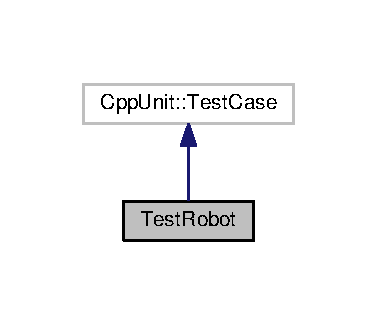
\includegraphics[width=181pt]{classTestRobot__inherit__graph}
\end{center}
\end{figure}


Graphe de collaboration de Test\+Robot\+:
\nopagebreak
\begin{figure}[H]
\begin{center}
\leavevmode
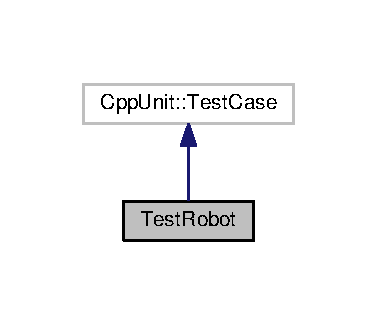
\includegraphics[width=181pt]{classTestRobot__coll__graph}
\end{center}
\end{figure}
\subsection*{Fonctions membres publiques}
\begin{DoxyCompactItemize}
\item 
\hypertarget{classTestRobot_a7a6f81e1509401afb6086073f142e059}{}{\bfseries Test\+Robot} (std\+::string name)\label{classTestRobot_a7a6f81e1509401afb6086073f142e059}

\item 
\hypertarget{classTestRobot_a29a7e512cf6a7c9871d0986f38ecd0ee}{}void {\bfseries set\+Up} ()\label{classTestRobot_a29a7e512cf6a7c9871d0986f38ecd0ee}

\item 
\hypertarget{classTestRobot_a8131b7d6df6b37c251c12c3a76a6f422}{}void {\bfseries test\+Deplacer} ()\label{classTestRobot_a8131b7d6df6b37c251c12c3a76a6f422}

\item 
\hypertarget{classTestRobot_a8131b7d6df6b37c251c12c3a76a6f422}{}void {\bfseries test\+Deplacer} ()\label{classTestRobot_a8131b7d6df6b37c251c12c3a76a6f422}

\item 
\hypertarget{classTestRobot_a8131b7d6df6b37c251c12c3a76a6f422}{}void {\bfseries test\+Deplacer} ()\label{classTestRobot_a8131b7d6df6b37c251c12c3a76a6f422}

\item 
\hypertarget{classTestRobot_a8131b7d6df6b37c251c12c3a76a6f422}{}void {\bfseries test\+Deplacer} ()\label{classTestRobot_a8131b7d6df6b37c251c12c3a76a6f422}

\item 
\hypertarget{classTestRobot_a8131b7d6df6b37c251c12c3a76a6f422}{}void {\bfseries test\+Deplacer} ()\label{classTestRobot_a8131b7d6df6b37c251c12c3a76a6f422}

\item 
\hypertarget{classTestRobot_a8131b7d6df6b37c251c12c3a76a6f422}{}void {\bfseries test\+Deplacer} ()\label{classTestRobot_a8131b7d6df6b37c251c12c3a76a6f422}

\item 
\hypertarget{classTestRobot_a8131b7d6df6b37c251c12c3a76a6f422}{}void {\bfseries test\+Deplacer} ()\label{classTestRobot_a8131b7d6df6b37c251c12c3a76a6f422}

\item 
\hypertarget{classTestRobot_a6d976a0403c5d0ad6ed217dc81fc52d9}{}void {\bfseries test\+Ouvrir} ()\label{classTestRobot_a6d976a0403c5d0ad6ed217dc81fc52d9}

\item 
\hypertarget{classTestRobot_a6d976a0403c5d0ad6ed217dc81fc52d9}{}void {\bfseries test\+Ouvrir} ()\label{classTestRobot_a6d976a0403c5d0ad6ed217dc81fc52d9}

\item 
\hypertarget{classTestRobot_a6d976a0403c5d0ad6ed217dc81fc52d9}{}void {\bfseries test\+Ouvrir} ()\label{classTestRobot_a6d976a0403c5d0ad6ed217dc81fc52d9}

\item 
\hypertarget{classTestRobot_a6d976a0403c5d0ad6ed217dc81fc52d9}{}void {\bfseries test\+Ouvrir} ()\label{classTestRobot_a6d976a0403c5d0ad6ed217dc81fc52d9}

\item 
\hypertarget{classTestRobot_a4bec25d19fc469f44c17e179f8f4ef7f}{}void {\bfseries test\+Ramasser} ()\label{classTestRobot_a4bec25d19fc469f44c17e179f8f4ef7f}

\item 
\hypertarget{classTestRobot_a4bec25d19fc469f44c17e179f8f4ef7f}{}void {\bfseries test\+Ramasser} ()\label{classTestRobot_a4bec25d19fc469f44c17e179f8f4ef7f}

\end{DoxyCompactItemize}


\subsection{Description détaillée}
Classe \hyperlink{classTestRobot}{Test\+Robot}. 

Tests de la classe \hyperlink{classRobot}{Robot} avec C\+P\+P\+Unit. \begin{DoxyAuthor}{Auteur}
Geoffrey D\+E\+S\+B\+R\+O\+S\+S\+E\+S 
\end{DoxyAuthor}
\begin{DoxyVersion}{Version}
1 
\end{DoxyVersion}
\begin{DoxyDate}{Date}
2015-\/12-\/10 
\end{DoxyDate}


La documentation de cette classe a été générée à partir du fichier suivant \+:\begin{DoxyCompactItemize}
\item 
Code\+Main/Test\+Robot.\+cpp\end{DoxyCompactItemize}

\hypertarget{classTileset}{}\section{Référence de la classe Tileset}
\label{classTileset}\index{Tileset@{Tileset}}
\subsection*{Fonctions membres publiques}
\begin{DoxyCompactItemize}
\item 
\hyperlink{classTileset_a9b75b605d834e3c9e25fb1c2429a36f6}{Tileset} ()
\begin{DoxyCompactList}\small\item\em Classe représentant un tileset, c\textquotesingle{}est-\/à-\/dire la liste des images utilisées pour dessiner la carte et leurs informations. \end{DoxyCompactList}\item 
\hyperlink{classTileset_ab9bd53a57698359f4ed3ff3d51370666}{Tileset} (clan\+::\+Image tilesheet, int h, int w, int tile\+\_\+h, int tile\+\_\+w, int spacing)
\item 
\hyperlink{classTileset_aa84d0a1454e7ca41989970371af95296}{Tileset} (clan\+::\+Image tilesheet, std\+::string tmx\+File)
\item 
\hyperlink{classTileset_a2a8acb9867fb31574cffa0c0ef8bd980}{Tileset} (const \hyperlink{classTileset}{Tileset} \&orig)
\item 
virtual \hyperlink{classTileset_afbb53f34f87b8b9c1f575349e89a6cd5}{$\sim$\+Tileset} ()
\item 
\hypertarget{classTileset_a81c24ec86c6b52a4f69f983571fecac5}{}int {\bfseries get\+Tile\+\_\+height} () const \label{classTileset_a81c24ec86c6b52a4f69f983571fecac5}

\item 
\hypertarget{classTileset_a3cf00412804a3f5210767cac1e0556eb}{}int {\bfseries get\+Tile\+\_\+width} () const \label{classTileset_a3cf00412804a3f5210767cac1e0556eb}

\item 
void \hyperlink{classTileset_a564a51b3a420ec234190e77e6b6acc1c}{draw\+Tile} (clan\+::\+Canvas c, int id, int x, int y)
\end{DoxyCompactItemize}


\subsection{Documentation des constructeurs et destructeur}
\hypertarget{classTileset_a9b75b605d834e3c9e25fb1c2429a36f6}{}\index{Tileset@{Tileset}!Tileset@{Tileset}}
\index{Tileset@{Tileset}!Tileset@{Tileset}}
\subsubsection[{Tileset}]{\setlength{\rightskip}{0pt plus 5cm}Tileset\+::\+Tileset (
\begin{DoxyParamCaption}
{}
\end{DoxyParamCaption}
)}\label{classTileset_a9b75b605d834e3c9e25fb1c2429a36f6}


Classe représentant un tileset, c\textquotesingle{}est-\/à-\/dire la liste des images utilisées pour dessiner la carte et leurs informations. 

\begin{DoxyAuthor}{Auteur}
Clément Bauchet 
\end{DoxyAuthor}
\begin{DoxyVersion}{Version}
1 
\end{DoxyVersion}
\begin{DoxyDate}{Date}
20 novembre 2015, 19\+:22
\end{DoxyDate}
Constructeur par défaut de la classe \hyperlink{classTileset}{Tileset}. \begin{DoxyReturn}{Renvoie}
\hyperlink{classTileset}{Tileset} un objet \hyperlink{classTileset}{Tileset} vide. 
\end{DoxyReturn}
\hypertarget{classTileset_ab9bd53a57698359f4ed3ff3d51370666}{}\index{Tileset@{Tileset}!Tileset@{Tileset}}
\index{Tileset@{Tileset}!Tileset@{Tileset}}
\subsubsection[{Tileset}]{\setlength{\rightskip}{0pt plus 5cm}Tileset\+::\+Tileset (
\begin{DoxyParamCaption}
\item[{clan\+::\+Image}]{tilesheet, }
\item[{int}]{h, }
\item[{int}]{w, }
\item[{int}]{tile\+\_\+h, }
\item[{int}]{tile\+\_\+w, }
\item[{int}]{spacing}
\end{DoxyParamCaption}
)}\label{classTileset_ab9bd53a57698359f4ed3ff3d51370666}
Constructeur de l\textquotesingle{}objet \hyperlink{classTileset}{Tileset}. 
\begin{DoxyParams}[1]{Paramètres}
\mbox{\tt in}  & {\em tilesheet} & l\textquotesingle{}image contenant les tiles \\
\hline
\mbox{\tt in}  & {\em h} & la hauteur du tileset en tiles \\
\hline
\mbox{\tt in}  & {\em w} & la largeur du tileset en tiles \\
\hline
\mbox{\tt in}  & {\em tile\+\_\+h} & la hauteur d\textquotesingle{}un tile en pixels \\
\hline
\mbox{\tt in}  & {\em tile\+\_\+w} & la largeur d\textquotesingle{}un tile en pixels \\
\hline
\mbox{\tt in}  & {\em spacing} & l\textquotesingle{}espace entre chaque tile dans la tilesheet, en pixels \\
\hline
\end{DoxyParams}
\begin{DoxyReturn}{Renvoie}
\hyperlink{classTileset}{Tileset} un objet \hyperlink{classTileset}{Tileset} avec les propriétés des valeurs en entrée. 
\end{DoxyReturn}
\hypertarget{classTileset_aa84d0a1454e7ca41989970371af95296}{}\index{Tileset@{Tileset}!Tileset@{Tileset}}
\index{Tileset@{Tileset}!Tileset@{Tileset}}
\subsubsection[{Tileset}]{\setlength{\rightskip}{0pt plus 5cm}Tileset\+::\+Tileset (
\begin{DoxyParamCaption}
\item[{clan\+::\+Image}]{tilesheet, }
\item[{std\+::string}]{tmx\+File}
\end{DoxyParamCaption}
)}\label{classTileset_aa84d0a1454e7ca41989970371af95296}
Constructeur de l\textquotesingle{}objet \hyperlink{classTileset}{Tileset}, par lecture du fichier de carte .tmx correspondant 
\begin{DoxyParams}[1]{Paramètres}
\mbox{\tt in}  & {\em tilesheet} & l\textquotesingle{}image contenant les tiles \\
\hline
\mbox{\tt in}  & {\em tmx\+File} & le nom du fichier de carte .tmx utilisant ce tileset \\
\hline
\end{DoxyParams}
\begin{DoxyReturn}{Renvoie}
\hyperlink{classTileset}{Tileset} un objet \hyperlink{classTileset}{Tileset} avec les propriétés récupérées depuis le fichier .tmx. 
\end{DoxyReturn}
\hypertarget{classTileset_a2a8acb9867fb31574cffa0c0ef8bd980}{}\index{Tileset@{Tileset}!Tileset@{Tileset}}
\index{Tileset@{Tileset}!Tileset@{Tileset}}
\subsubsection[{Tileset}]{\setlength{\rightskip}{0pt plus 5cm}Tileset\+::\+Tileset (
\begin{DoxyParamCaption}
\item[{const {\bf Tileset} \&}]{orig}
\end{DoxyParamCaption}
)}\label{classTileset_a2a8acb9867fb31574cffa0c0ef8bd980}
Constructeur de l\textquotesingle{}objet \hyperlink{classTileset}{Tileset} par copie d\textquotesingle{}un autre tileset \begin{DoxyReturn}{Renvoie}
\hyperlink{classTileset}{Tileset} un objet \hyperlink{classTileset}{Tileset} identique à celui fourni en entrée 
\end{DoxyReturn}
\hypertarget{classTileset_afbb53f34f87b8b9c1f575349e89a6cd5}{}\index{Tileset@{Tileset}!````~Tileset@{$\sim$\+Tileset}}
\index{````~Tileset@{$\sim$\+Tileset}!Tileset@{Tileset}}
\subsubsection[{$\sim$\+Tileset}]{\setlength{\rightskip}{0pt plus 5cm}Tileset\+::$\sim$\+Tileset (
\begin{DoxyParamCaption}
{}
\end{DoxyParamCaption}
)\hspace{0.3cm}{\ttfamily [virtual]}}\label{classTileset_afbb53f34f87b8b9c1f575349e89a6cd5}
Destructeur de \hyperlink{classTileset}{Tileset} 

\subsection{Documentation des fonctions membres}
\hypertarget{classTileset_a564a51b3a420ec234190e77e6b6acc1c}{}\index{Tileset@{Tileset}!draw\+Tile@{draw\+Tile}}
\index{draw\+Tile@{draw\+Tile}!Tileset@{Tileset}}
\subsubsection[{draw\+Tile}]{\setlength{\rightskip}{0pt plus 5cm}void Tileset\+::draw\+Tile (
\begin{DoxyParamCaption}
\item[{clan\+::\+Canvas}]{c, }
\item[{int}]{id, }
\item[{int}]{x, }
\item[{int}]{y}
\end{DoxyParamCaption}
)}\label{classTileset_a564a51b3a420ec234190e77e6b6acc1c}
Méthode dessinant une case du tileset à une position donnée 
\begin{DoxyParams}[1]{Paramètres}
\mbox{\tt in}  & {\em c} & le canvas où dessiner la case \\
\hline
\mbox{\tt in}  & {\em id} & le numéro dans le tileset de la tile à dessiner \\
\hline
\mbox{\tt in}  & {\em x} & la coordonnée x de la position où dessiner la case \\
\hline
\mbox{\tt in}  & {\em y} & la coordonnée y de la position où dessiner la case \\
\hline
\end{DoxyParams}


La documentation de cette classe a été générée à partir des fichiers suivants \+:\begin{DoxyCompactItemize}
\item 
Code\+Main/tileset.\+hpp\item 
Code\+Main/tileset.\+cpp\end{DoxyCompactItemize}

%--- End generated contents ---

% Index
\backmatter
\newpage
\phantomsection
\clearemptydoublepage
\addcontentsline{toc}{chapter}{Index}
\printindex

\end{document}
